\documentclass[12pt]{article}

\usepackage[margin=1.0in]{geometry}
\usepackage[parfill]{parskip}
\usepackage{amsmath}
\usepackage{amssymb}
\usepackage{amsthm}
\usepackage{graphicx}
\usepackage[font=bf]{caption}
\usepackage{changepage}



%-------------------------------------------------------------------------------
\begin{document}
%-------------------------------------------------------------------------------



\setlength{\parskip}{12pt}      % set paragraph skipping to one whole line
\setlength{\tabcolsep}{12pt}    % give some room between table columns
\hfuzz=60pt                     % give a little margin room for the double-column tables



% establish a condensed itemized list format
\newenvironment{myitemize}
{ \begin{itemize}
    \setlength{\itemsep}{0pt}
    \setlength{\parskip}{0pt}
    \setlength{\parsep}{0pt}     }
{ \end{itemize}                  } 



% establish theorem and lemma formats
\newtheorem{theorem}{Theorem}[section]
\newtheorem{lemma}[theorem]{Lemma}



\begin{titlepage}
    \begin{center}
        \vspace*{\fill}
        
        \huge
        The Kalman Filter \\
        
        \large
        An Adventure in Derivation
        
        \vspace{24pt}
        
        \large
        Robert S. Huston \\
        Pinpoint Dynamics, LLC \\
        
        \vspace{24pt}
        
        \today
        
        \vspace{24pt}
        
        \large
        Copyright © 2024, 2025 Robert S. Huston. All rights reserved.
        
        \vfill
    \end{center}
\end{titlepage}



\begin{abstract}
This document presents an assorted collection of derivations and notes pertaining to the
Kalman filter. They are targeted to the practicing engineer who has been tasked with
developing and implementing a Kalman filtering solution. The mathematical derivations are
intended to eliminate the mysteries of how and why the Kalman filter works. In addition,
the document presents the various versions of the Kalman filter and offers some key
implementation strategies.
\end{abstract}



\clearpage



\begin{adjustwidth}{1in}{1in}
    \vspace*{\fill}
    
    \textit{
        So I jump ship in Hong Kong and I make my way over to Tibet, and I get on as a
        looper at a course over in the Himalayas.
        A looper, you know, a caddy, a looper, a jock. So, I tell them I'm a pro jock,
        and who do you think they give me? The Dalai Lama, himself. Twelfth son of the Lama.
        The flowing robes, the grace, bald...striking. So, I'm on the first tee with him.
        I give him the driver. He hauls off and whacks one - big hitter, the Lama - long,
        into a ten-thousand foot crevasse, right at the base of this glacier.
        Do you know what the Lama says? "Gunga galunga...gunga, gunga-lagunga."
        So we finish the eighteenth and he's gonna stiff me. And I say, "Hey, Lama, hey,
        how about a little something, you know, for the effort, you know."
        And he says, "Oh, uh, there won't be any money, but when you die, on your deathbed,
        you will receive total consciousness." So I got that goin' for me, which is nice.
    }
    
    - Carl Spackler (Bill Murray, "Caddyshack" - 1980)
    
    \vfill
\end{adjustwidth}



\clearpage



\tableofcontents



\clearpage



%-------------------------------------------------------------------------------
\section{Introduction}
%-------------------------------------------------------------------------------

Consider the discrete-time linear system dynamical process model and linear observation model

\begin{equation*}
    \begin{aligned}
        \mathbf{x}_{k+1} &= \mathbf{\Phi}_{k+1|k} \mathbf{x}_k + \mathbf{u}_k + \mathbf{\Gamma}_{k+1|k} \mathbf{w}_k \\
        \mathbf{z}_k &= \mathbf{H}_k \mathbf{x}_k + \mathbf{v}_k
    \end{aligned}
\end{equation*}

where $\mathbf{x}$ is an $n \times 1$ state vector,
$\mathbf{\Phi}$ is an $n \times n$ state transition matrix,
$\mathbf{u}$ is an $n \times 1$ control input,
$\mathbf{\Gamma}$ is an $n \times p$ disturbance distribution matrix,
and $\mathbf{w}$ is a $p \times 1$ white process noise sequence of random disturbances with covariance

\begin{equation*}
    E \left\{ \mathbf{w}_k \mathbf{w}_k^T \right\} = \mathbf{Q}_k
\end{equation*}

and where $\mathbf{z}$ is an $m \times 1$ observation vector,
$\mathbf{H}$ is an $m \times n$ observation transformation matrix,
and $\mathbf{v}_k$ is an $m \times 1$ white error noise sequence of random observation errors with covariance

\begin{equation*}
    E \left\{ \mathbf{v}_k \mathbf{v}_k^T \right\} = \mathbf{R}_k
\end{equation*}

and where both the process and observation noise sequences are uncorrelated

\begin{equation*}
    E \left\{ \mathbf{w}_j \mathbf{v}_k^T \right\} = \mathbf{0} \, , \phantom{.} \mathrm{for} \, \mathrm{all} \, j \, \mathrm{and} \, k
\end{equation*}

Figure \ref{fig:dt-linear-system} diagrammatically depicts the linear system model.

\begin{figure}[ht]
    \centering
    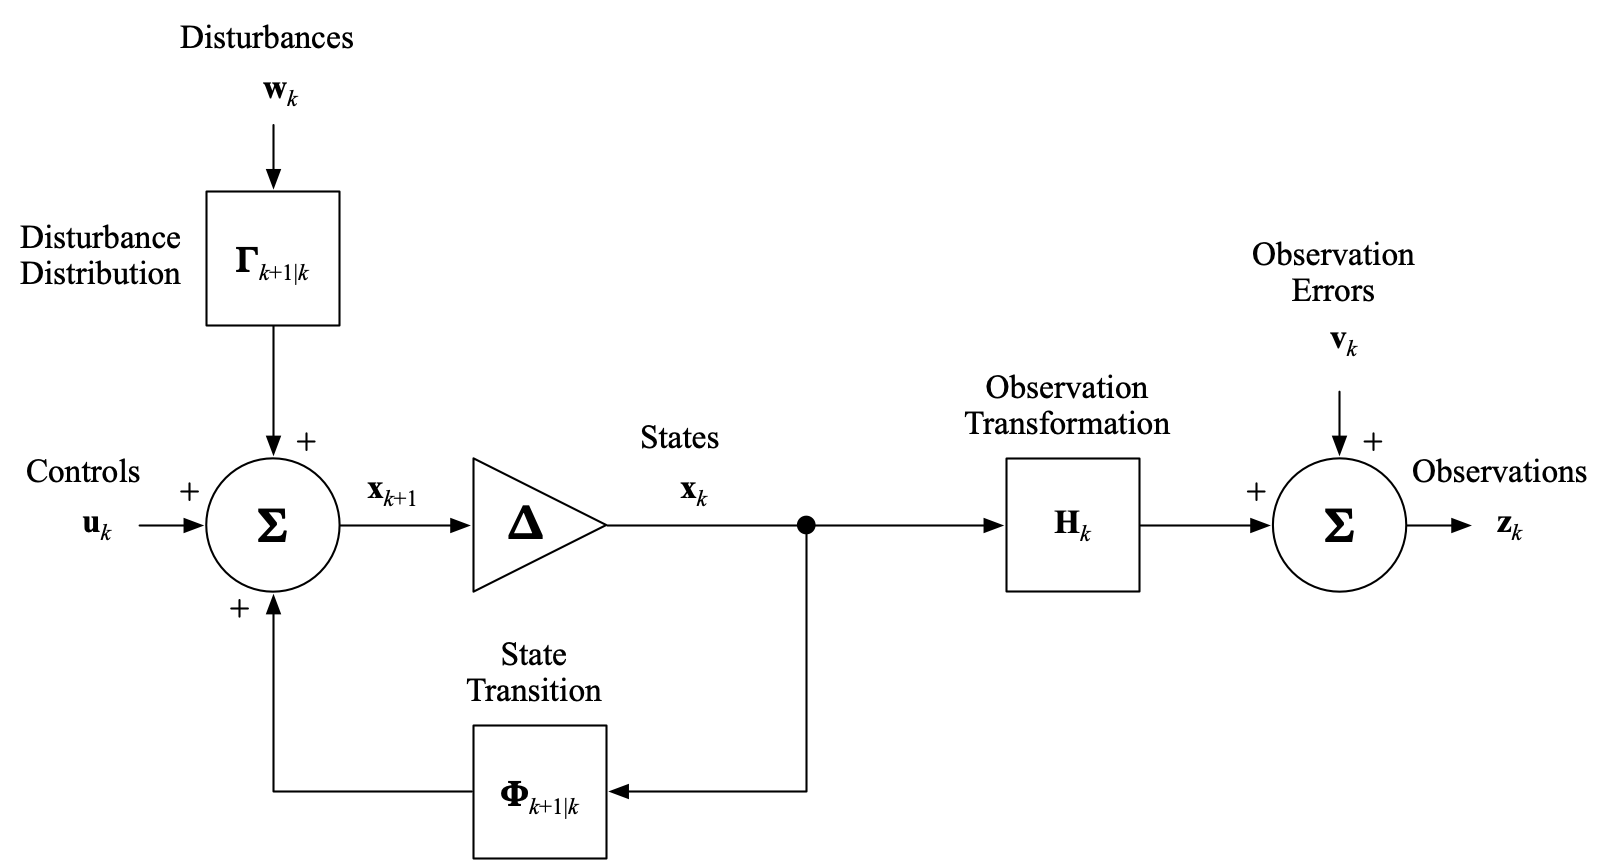
\includegraphics[width=0.95\textwidth]{images/DT-Linear-System.png}
    \caption{Discrete-Time Linear System}
    \label{fig:dt-linear-system}
\end{figure}

Given the observations, $\mathbf{z}_k$,
the modeling knowledge of $\mathbf{\Phi}_{k+1|k}$, $\mathbf{\Gamma}_{k+1|k}$, and $\mathbf{H}_k$,
and the statistical characteristics of $\mathbf{w}_k$ and $\mathbf{v}_k$,
the Kalman filter provides an optimal estimate of the state, $\mathbf{x}_k$, at time event $k$

\begin{equation*}
    \hat{\mathbf{x}}_k = E \left\{ \mathbf{x}_k \right\}
\end{equation*}

with a state estimation error

\begin{equation*}
    \mathbf{e}_k = \mathbf{x}_{k} - \hat{\mathbf{x}}_k
\end{equation*}

and where the covariance of the state estimation error is

\begin{equation*}
    \begin{aligned}
        \mathbf{P}_k &= E \left\{ \mathbf{e}_k \mathbf{e}_k^T \right\} \\
        &= E \left\{ \left[ \mathbf{x}_{k} - \hat{\mathbf{x}}_k \right] \left[ \mathbf{x}_{k} - \hat{\mathbf{x}}_k \right]^T \right\}
    \end{aligned}
\end{equation*}

The well-known Kalman filter recurrence update cycle is comprised of two steps:
a "projection" or \textit{a priori} update, and a "correction" or \textit{a posteriori} update.

I. Projection (\textit{a priori}) update:

\begin{equation*}
    \begin{aligned}
        \hat{\mathbf{x}}_{k|k-1} &= \mathbf{\Phi}_{k|k-1} \hat{\mathbf{x}}_{k-1} + \mathbf{u}_{k-1} \\
        \mathbf{P}_{k|k-1} &= \mathbf{\Phi}_{k|k-1} \mathbf{P}_{k-1} \mathbf{\Phi}_{k|k-1}^T + \mathbf{\Gamma}_{k|k-1} \mathbf{Q}_{k-1} \mathbf{\Gamma}_{k|k-1}^T
    \end{aligned}
\end{equation*}

II. Correction (\textit{a posteriori}) update:

\begin{equation*}
    \begin{aligned}
        \hat{\mathbf{z}}_k &= \mathbf{H}_k \hat{\mathbf{x}}_{k|k-1} \\
        \tilde{\mathbf{z}}_k &= \mathbf{z}_k - \hat{\mathbf{z}}_k \\
        \mathbf{S}_k &= \mathbf{H}_k \mathbf{P}_{k|k-1} \mathbf{H}_k^T + \mathbf{R}_k \\
        \mathbf{K}_k &= \mathbf{P}_{k|k-1} \mathbf{H}_{k}^T \mathbf{S}_k^{-1} \\
        \hat{\mathbf{x}}_k &= \hat{\mathbf{x}}_{k|k-1} +\mathbf{K}_k \tilde{\mathbf{z}}_k \\
        \mathbf{P}_k &= \left[ \mathbf{I} - \mathbf{K}_k \mathbf{H}_k \right] \mathbf{P}_{k|k-1}
    \end{aligned}
\end{equation*}

Figure \ref{fig:kf-diagram} diagrammatically depicts the Kalman filter.

\begin{figure}[ht]
    \centering
    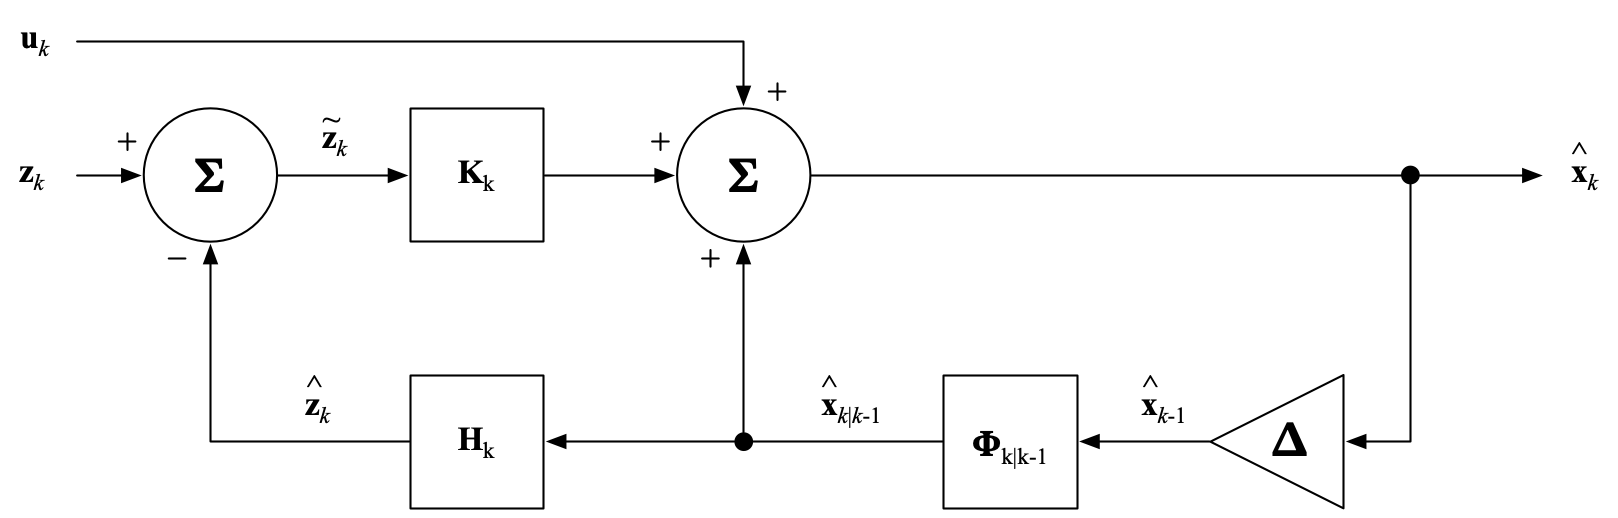
\includegraphics[width=0.95\textwidth]{images/KF-Diagram.png}
    \caption{Kalman Filter Diagram}
    \label{fig:kf-diagram}
\end{figure}

Unfortunately, the vast literature for the Kalman filter, and its varieties, can be
overwhelmingly confounding. Different variables are used. Different notations are used.
Different terms are used. The complexity of some of the mathematical proofs and theorems
can obscure the more important matters.

And then there are questions \ldots many questions.
What’s with all these equations?
What makes them so special?
Where do they come from?
What is meant by "optimal" gain?
Why can’t I just use least-squares estimation?
Isn’t the Kalman filter just a specialized least-squares filter anyway?
What does it mean when it is said that "$\mathbf{S}_k$" represents the covariance of the observation error?
Why are there so many different forms of the filter, and which one should I use?
And did Jeffrey Epstein really kill himself?

This document is an assorted collection of derivations and notes pertaining to the Kalman
filter. They are targeted to the practicing engineer who has been tasked with developing
and implementing a Kalman filtering solution. The mathematical derivations are therefore
intended to eliminate some of the mysteries of how and why the Kalman filter works, as
well as what the various versions and implementation strategies have to offer.

Some assumptions are made about the reader:

\begin{myitemize}
    \item The reader understands basic matrix algebra
    \item The reader understands basic calculus
    \item The reader understands basic probability and statistics
\end{myitemize}

Lastly, this document is written the the way I wished I could have experienced when I was
first learning the Kalman filter. Hopefully, it is helpful to the reader as is.
If not, well then too bad.

\clearpage



%-------------------------------------------------------------------------------
\section{Conventions and Notations}
%-------------------------------------------------------------------------------

When I began my journey into studying the Kalman filter, my primary reference was the
"Robert Grover Brown" book \cite{rgbrown1983}, and much of my choice of conventions and
notations comes from that book. I also heavily relied on Sorenson’s material
\cite{sorenson1985} which was consistent with R.G. Brown notation. As I accumulated other
references over the years, I discovered that the Brown/Sorenson conventions and notations
were dominant. Granted there are other conventions and notations in the Kalman filtering
literature, but I feel most at home when using the Brown/Sorenson conventions and notations,
and those are the ones I’ve chosen to adopt in this document.

In particular, $\mathbf{x}_k$ represents a system state vector at time event "$k$",
$\mathbf{\Phi}_{k+1|k}$ represents a linear state transition matrix that transitions the
state from time events "$k$" to "$k+1$",
$\mathbf{z}_k$ represents an observation (i.e., measurement) vector that observes the
system output at time event "$k$",
and $\mathbf{H}_k$ represents a linear observation transformation from $\mathbf{x}_k$
to $\mathbf{z}_k$.
Additionally, $\mathbf{w}_k$ and $\mathbf{v}_k$ represent random sequences that model the
system dynamics variations and observation variations, respectively, with covariances
$\mathbf{Q}_k$ and $\mathbf{R}_k$, respectively.
Lastly, the system state estimation error covariance is represented by $\mathbf{P}_k$.

In addition to the many different choices of variables in the technical literature, there
are also many notational styles.
For instance, instead of using the "$k$" and "$k+1|k$" subscripts, some references use
functional forms instead, as in "$\mathbf{x}(k)$" and "$\mathbf{\Phi}(k+1|k)$".
Others use "$+$" and "$-$" indicators to differentiate \textit{a priori} variables from
\textit{a posteriori} variables, e.g., $\mathbf{P}_k^-$ instead of $\mathbf{P}_{k|k-1}$,
and $\mathbf{P}_k^+$ instead of $\mathbf{P}_{k|k}$.
The notations adopted in this document strive to make the equations clear (or as clear
as they can be) without being "too busy" in the variable descriptors;
$\mathbf{\Phi}_{k+1|k}$ is more readable in an expression than $\mathbf{\Phi}(k+1|k)$.

There are many references that do not distinguish visually between a scalar quantity and
a matrix quantity. While this may have been a necessity in the days of typewriters and
early word processors, it also does the reader an extreme disservice. Knowing that a
variable is a scalar or a matrix is fundamental in the understanding of an equation or
derivation, and given today’s technology in word processing and electronic typesetting,
there is no excuse for not adhering to the accepted conventions where an italic variable,
$s$, is a scalar quantity, and a boldface variable, $\mathbf{M}$, is a matrix quantity.

I’ve often wondered why this particular choice of variables was picked by certain authors.
For instance, why use $\mathbf{z}$ for the observation vector when the state vector is
$\mathbf{x}$ and the natural choice would be to use $\mathbf{y}$ instead? After all,
that’s what all the classical linear control system theory resources use. And why use
$\mathbf{H}$ as the linear observation transformation instead of something more consistent
with classical linear control system theory? My uneducated guess is that using $\mathbf{z}$
allows for the use of $\mathbf{y}$ to represent additional state values (e.g., hidden
states) in augmented system formulations, and using $\mathbf{H}$ is simply a natural
alphabetic progression after $\mathbf{F}$ and $\mathbf{G}$ are assigned for discrete-time
system functional transformations. For instance, consider the classical continuous-time
linear system description:

\begin{equation*}
    \begin{aligned}
        \mathbf{\dot{x}} &= \mathbf{A} \mathbf{x} + \mathbf{B} \mathbf{u} \\
        \mathbf{y} &= \mathbf{C} \mathbf{x} + \mathbf{D} \mathbf{u} \\
    \end{aligned}
\end{equation*}

where $\mathbf{x}$ is the system state, $\mathbf{u}$ is the control input, and $\mathbf{y}$
is the output observation. In transforming to a discrete-time description, a natural
choice of variables would be

\begin{equation*}
    \begin{aligned}
        \mathbf{x}_{k+1} &= \mathbf{F}_k \mathbf{x}_k + \mathbf{G}_k \mathbf{u}_k \\
        \mathbf{z}_k &= \mathbf{H}_k \mathbf{x}_k + \mathbf{J}_k \mathbf{u}_k
    \end{aligned}
\end{equation*}

We should stay away from using $\mathbf{E}$ because it could easily be confused with the
expectation operation $E \left\{ \cdots \right\}$, and we can’t use $\mathbf{I}$ because
that’s the identity matrix (although I’ve seen some authors use $\mathbf{I}_k$ to represent
an information matrix value at time event "$k$", causing me horrible confusion), so the
choices of $\mathbf{H}$ seems to make logical sense. Similarly, the choices for covariance
values appear to be alphabetically assigned. If $\mathbf{P}$ is our first-assigned covariance,
then using $\mathbf{Q}$ and $\mathbf{R}$ make sense for the next two assignments. Of course,
this reasoning behind the assignments is pure conjecture on my part, but it allows me to
find order in the conventions that I’ve chosen from R.G. Brown and others.

The following list summarizes the general conventions and notations used in this document:

\begin{myitemize}
    \item An italic variable, $s$, designates a scalar quantity (the variable can be of any case)
    \item A boldface lower-case variable, $\mathbf{v}$, designates a vector matrix quantity
    \item A boldface upper-case variable, $\mathbf{M}$, designates a block matrix quantity
    \item $\mathbf{x}_k$ designates a system state vector at time event "$k$"
    \item $\hat{\mathbf{x}}_k$ designates an estimate of the system state vector, $\mathbf{x}_k$, at time event "$k$"
    \item $\mathbf{P}_k$ designates the covariance matrix of the state estimation error, $\mathbf{x}_k - \hat{\mathbf{x}}_k$
    \item $\mathbf{\Phi}_{k+1|k}$ designates a linear state transition matrix that transitions $\mathbf{x}_k$ from time events "$k$" to "$k+1$"
    \item $\mathbf{u}_k$ designates a system control input vector at time event "$k$"
    \item $\mathbf{w}_k$ designates a system process random variation vector at time event "$k$"
    \item $\mathbf{Q}_k$ designates the covariance matrix of the system process random variation, $\mathbf{w}_k$
    \item $\mathbf{\Gamma}_{k+1|k}$ designates a linear matrix that transforms $\mathbf{w}_k$ from time events "$k$" to "$k+1$" into the state space of $\mathbf{x}_k$
    \item $\mathbf{z}_k$ designates an observation (i.e., measurement) vector that observes the system at time event "$k$"
    \item $\hat{\mathbf{z}}_k$ designates an estimate of the observation vector, $\mathbf{z}_k$, at time event "$k$"
    \item $\mathbf{R}_k$ designates the covariance matrix of the observation estimation error, $\mathbf{z}_k - \hat{\mathbf{z}}_k$
    \item $\mathbf{H}_k$ designates a linear observation transformation matrix from the state space of $\mathbf{x}_k$ into the state space of $\mathbf{z}_k$
    \item $\mathbf{v}_k$ designates an observation random variation vector at time event "$k$"
    \item $\mathbf{R}_k$ designates the covariance matrix of the observation random variation, $\mathbf{v}_k$
    \item $\mathbf{K}_k$ designates the state estimation filter gain matrix, i.e., the Kalman gain
\end{myitemize}


\clearpage



%-------------------------------------------------------------------------------
\section{Weighted Least-Squares Estimation}
%-------------------------------------------------------------------------------

Consider the overdetermined observation system

\begin{equation*}
    \mathbf{z} = \mathbf{H} \mathbf{x} + \mathbf{v}
\end{equation*}

where $\mathbf{z}$ is an $m \times 1$ observation vector,
$\mathbf{x}$ is an $m \times 1$ state vector,
$\mathbf{H}$ is an $m \times n$ observation matrix,
and $\mathbf{v}$ is an $m \times 1$ random vector of observation errors with covariance

\begin{equation*}
    E \left\{ \mathbf{v} \mathbf{v}^T \right\} = \mathbf{R}
\end{equation*}

As stated previously, $m \ge n$, i.e., there can be more observations than there are states.
So $\mathbf{H}$ is not necessarily square:

\begin{equation*}
    \begin{bmatrix}
    z_1 \\
    z_2 \\
    z_3 \\
    z_4 \\
    z_5 \\
    \vdots \\
    z_m
    \end{bmatrix}
    =
    \begin{bmatrix}
    h_{11} & h_{12} & h_{13} & \dots & h_{1n} \\
    h_{21} & h_{22} & h_{23} & \dots & h_{2n} \\
    h_{31} & h_{32} & h_{33} & \dots & h_{3n} \\
    h_{41} & h_{42} & h_{43} & \dots & h_{4n} \\
    h_{51} & h_{52} & h_{53} & \dots & h_{5n} \\
    \vdots & \vdots & \vdots & \ddots & \vdots \\
    h_{m1} & h_{m2} & h_{m3} & \dots & h_{mn}
    \end{bmatrix}
    \begin{bmatrix}
    x_1 \\
    x_2 \\
    x_3 \\
    \vdots \\
    x_n
    \end{bmatrix}
    +
    \begin{bmatrix}
    v_1 \\
    v_2 \\
    v_3 \\
    v_4 \\
    v_5 \\
    \vdots \\
    v_m
    \end{bmatrix}
\end{equation*}

Assume that we already have a state estimate, $\hat{\mathbf{x}}$. We can then determine the
corresponding observation estimate, $\hat{\mathbf{z}}$, from

\begin{equation*}
    \hat{\mathbf{z}} = \mathbf{H} \hat{\mathbf{x}}
\end{equation*}

We form the observation residual, i.e., the observation error

\begin{equation*}
    \tilde{\mathbf{z}} = \mathbf{z} - \hat{\mathbf{z}}
\end{equation*}

We can then form the weighted squared error term

\begin{equation*}
    \epsilon^2 = \tilde{\mathbf{z}}^T \mathbf{W} \tilde{\mathbf{z}}
\end{equation*}

where $\mathbf{W}$ is an arbitrary symmetric weighting matrix.

The objective is to determine the "best" value for $\hat{\mathbf{x}}$ that fits the
observation data $\mathbf{z}$. We will define "best" to be the value of $\hat{\mathbf{x}}$
that minimizes $\epsilon^2$. In other words, we want to find the "least-squares"
estimate of $\mathbf{x}$.

Expanding the terms of $\epsilon^2$ gives

\begin{equation*}
    \begin{aligned}
        \epsilon^2 &= \tilde{\mathbf{z}}^T \mathbf{W} \tilde{\mathbf{z}} \\
                   &= \left[ \mathbf{z} - \hat{\mathbf{z}} \right]^T \mathbf{W} \left[ \mathbf{z} - \hat{\mathbf{z}} \right] \\
                   &= \left[ \mathbf{z} - \mathbf{H} \hat{\mathbf{x}} \right]^T \mathbf{W} \left[ \mathbf{z} - \mathbf{H} \hat{\mathbf{x}} \right] \\
                   &= \left[ \mathbf{z}^T - \hat{\mathbf{x}}^T \mathbf{H}^T \right] \mathbf{W} \left[ \mathbf{z} - \mathbf{H} \hat{\mathbf{x}} \right] \\
                   &= \mathbf{z}^T \mathbf{W} \mathbf{z} - \hat{\mathbf{x}}^T \mathbf{H}^T \mathbf{W} \mathbf{z}
                      - \mathbf{z}^T \mathbf{W} \mathbf{H} \hat{\mathbf{x}} + \hat{\mathbf{x}}^T \mathbf{H}^T \mathbf{W} \mathbf{H} \hat{\mathbf{x}}
    \end{aligned}
\end{equation*}

To find the value of $\hat{\mathbf{x}}$ that minimizes $\epsilon^2$, we differentiate 
$\epsilon^2$ with respect to $\hat{\mathbf{x}}$ and set the resulting expression to zero.
We can make use of the following differentiation formulas:

\begin{equation*}
    \frac{ d \left( \mathbf{a}^T \mathbf{x} \right) }{d \mathbf{x}} = \frac{ d \left( \mathbf{x}^T \mathbf{a} \right) }{d \mathbf{x}} = \mathbf{a}
\end{equation*}

\begin{equation*}
    \frac{ d \left( \mathbf{x}^T \mathbf{A} \mathbf{x} \right) }{d \mathbf{x}} = 2 \mathbf{A} \mathbf{x} \, , \phantom{X} (\mathbf{A} \, \mathrm{is} \, \mathrm{symmetric})
\end{equation*}

We use the differential operation where, if $s$ is a scalar value and $\mathbf{x}$ is a
column vector value, then

\begin{equation*}
    \frac {d s} {d \mathbf{x}} \triangleq
    \begin{bmatrix}
    \dfrac{\partial s}{\partial x_{1}} \\
    \phantom{.} \\
    \dfrac{\partial s}{\partial x_{2}} \\
    \phantom{.} \\
    \dfrac{\partial s}{\partial x_{3}} \\
    \phantom{.} \\
    \vdots
    \end{bmatrix}
\end{equation*}

Then

\begin{equation*}
    \begin{aligned}
        \frac{ d \left( \epsilon^2 \right) }{d \hat{\mathbf{x}}}
        &= - \mathbf{H}^T \mathbf{W} \mathbf{z}
           - \left( \mathbf{z}^T \mathbf{W} \mathbf{H} \right)^T
           + 2 \mathbf{H}^T \mathbf{W} \mathbf{H} \hat{\mathbf{x}} \\
        &= \mathbf{0}
    \end{aligned}
\end{equation*}

and so, observing that $\mathbf{H}^T \mathbf{W} \mathbf{H}$ is invertible, we see that

\begin{equation*}
    \begin{aligned}
        - \mathbf{H}^T \mathbf{W} \mathbf{z}
        -  \left( \mathbf{z}^T \mathbf{W} \mathbf{H} \right)^T
        + 2 \mathbf{H}^T \mathbf{W} \mathbf{H} \hat{\mathbf{x}}
        &= \mathbf{0} \\
        - \mathbf{H}^T \mathbf{W} \mathbf{z}
        - \mathbf{H}^T \mathbf{W} \mathbf{z}
        + 2 \mathbf{H}^T \mathbf{W} \mathbf{H} \hat{\mathbf{x}}
        &= \mathbf{0} \\
        - 2 \mathbf{H}^T \mathbf{W} \mathbf{z}
        + 2 \mathbf{H}^T \mathbf{W} \mathbf{H} \hat{\mathbf{x}}
        &= \mathbf{0} \\
        \mathbf{H}^T \mathbf{W} \mathbf{H} \hat{\mathbf{x}} &= \mathbf{H}^T \mathbf{W} \mathbf{z} \\
        \hat{\mathbf{x}} &= \left( \mathbf{H}^T \mathbf{W} \mathbf{H} \right)^{-1} \mathbf{H}^T \mathbf{W} \mathbf{z} \\
    \end{aligned}
\end{equation*}

Hence the "best" value of $\hat{\mathbf{x}}$ that fits the observation data $\mathbf{z}$
in the least-squares sense is

\boxed{
\parbox{\textwidth}{
\begin{equation}
    \hat{\mathbf{x}} = \left( \mathbf{H}^T \mathbf{W} \mathbf{H} \right)^{-1} \mathbf{H}^T \mathbf{W} \mathbf{z}
\end{equation}
}
}

To find the optimal value of $\mathbf{W}$, we form the state estimation error

\begin{equation*}
    \begin{aligned}
        \mathbf{e} &= \mathbf{x} - \hat{\mathbf{x}} \\
        &= \mathbf{x} - \left( \mathbf{H}^T \mathbf{W} \mathbf{H} \right)^{-1} \mathbf{H}^T \mathbf{W} \mathbf{z} \\
        &= \mathbf{x} - \left( \mathbf{H}^T \mathbf{W} \mathbf{H} \right)^{-1} \mathbf{H}^T \mathbf{W} \left[ \mathbf{H} \mathbf{x} + \mathbf{v} \right] \\
        &= \mathbf{x}
           - \left( \mathbf{H}^T \mathbf{W} \mathbf{H} \right)^{-1} \mathbf{H}^T \mathbf{W} \mathbf{H} \mathbf{x}
           - \left( \mathbf{H}^T \mathbf{W} \mathbf{H} \right)^{-1} \mathbf{H}^T \mathbf{W} \mathbf{v} \\
        &= \mathbf{x} - \mathbf{x}
           - \left( \mathbf{H}^T \mathbf{W} \mathbf{H} \right)^{-1} \mathbf{H}^T \mathbf{W} \mathbf{v} \\
        &= - \left( \mathbf{H}^T \mathbf{W} \mathbf{H} \right)^{-1} \mathbf{H}^T \mathbf{W} \mathbf{v} \\
    \end{aligned}
\end{equation*}

Then the covariance of the state estimation error is

\begin{equation*}
    \begin{aligned}
        \mathbf{P} &= E \left\{ \mathbf{e} \, \mathbf{e}^T \right\} \\
        &= E \left\{ \left[ - \left( \mathbf{H}^T \mathbf{W} \mathbf{H} \right)^{-1} \mathbf{H}^T \mathbf{W} \mathbf{v} \right]
           \left[ - \left( \mathbf{H}^T \mathbf{W} \mathbf{H} \right)^{-1} \mathbf{H}^T \mathbf{W} \mathbf{v} \right]^T \right\} \\
        &= E \left\{ \left[ - \left( \mathbf{H}^T \mathbf{W} \mathbf{H} \right)^{-1} \mathbf{H}^T \mathbf{W} \mathbf{v} \right]
           \left[ - \mathbf{v}^T \mathbf{W} \mathbf{H} \left( \mathbf{H}^T \mathbf{W} \mathbf{H} \right)^{-1} \right] \right\} \\
        &= E \left\{ \left( \mathbf{H}^T \mathbf{W} \mathbf{H} \right)^{-1} \mathbf{H}^T \mathbf{W} \mathbf{v}
           \mathbf{v}^T \mathbf{W} \mathbf{H} \left( \mathbf{H}^T \mathbf{W} \mathbf{H} \right)^{-1} \right\} \\
        &= \left( \mathbf{H}^T \mathbf{W} \mathbf{H} \right)^{-1} \mathbf{H}^T \mathbf{W}
           \;\, E \left\{ \mathbf{v} \mathbf{v}^T \right\} \;
           \mathbf{W} \mathbf{H} \left( \mathbf{H}^T \mathbf{W} \mathbf{H} \right)^{-1} \\
        &= \left( \mathbf{H}^T \mathbf{W} \mathbf{H} \right)^{-1} \mathbf{H}^T \mathbf{W}
           \mathbf{R}
           \mathbf{W} \mathbf{H} \left( \mathbf{H}^T \mathbf{W} \mathbf{H} \right)^{-1} \\
    \end{aligned}
\end{equation*}

In order to simplify this expression, we set $\mathbf{R} = \mathbf{W}^{-1}$. Then

\begin{equation*}
    \begin{aligned}
        \mathbf{P}
        &= \left( \mathbf{H}^T \mathbf{W} \mathbf{H} \right)^{-1}
           \mathbf{H}^T \mathbf{W} \mathbf{R} \mathbf{W} \mathbf{H}
           \left( \mathbf{H}^T \mathbf{W} \mathbf{H} \right)^{-1} \\
        &= \left( \mathbf{H}^T \mathbf{W} \mathbf{H} \right)^{-1}
           \mathbf{H}^T \mathbf{W} \mathbf{W}^{-1} \mathbf{W} \mathbf{H}
           \left( \mathbf{H}^T \mathbf{W} \mathbf{H} \right)^{-1} \\
        &= \left( \mathbf{H}^T \mathbf{W} \mathbf{H} \right)^{-1}
           \mathbf{H}^T \mathbf{W} \mathbf{H}
           \left( \mathbf{H}^T \mathbf{W} \mathbf{H} \right)^{-1} \\
        &= \left( \mathbf{H}^T \mathbf{W} \mathbf{H} \right)^{-1}  \\
    \end{aligned}
\end{equation*}

Hence, the optimal value for $\mathbf{W}$ is

\boxed{
\parbox{\textwidth}{
\begin{equation}
    \mathbf{W} = \mathbf{R}^{-1}
\end{equation}
}
}

Note that the least-squares solution only uses information from the observation
description. It has no knowledge of the system state dynamics.

Let us now consider the unweighted ($\mathbf{W} = \mathbf{I}$) least-squares solution

\begin{equation*}
    \hat{\mathbf{x}} = \left( \mathbf{H}^T \mathbf{H} \right)^{-1} \mathbf{H}^T \mathbf{z}
\end{equation*}

Define

\begin{equation*}
    \mathbf{A} = \left( \mathbf{H}^T \mathbf{H} \right)^{-1} \mathbf{H}^T
\end{equation*}

so that

\begin{equation*}
    \hat{\mathbf{x}} = \mathbf{A} \mathbf{z}
\end{equation*}

If, for the moment, let us treat the vector $\mathbf{z}$ as a zero-mean Gaussian random
vector with unit noise covariance,

\begin{equation*}
    E \left\{ \mathbf{z} \, \mathbf{z}^T \right\} = \mathbf{I}
\end{equation*}

then, because the solution for $\hat{\mathbf{x}}$ is a linear transformation on
$\mathbf{z}$, the covariance of $\hat{\mathbf{x}}$ is then

\begin{equation*}
    \begin{aligned}
        E \left\{ \hat{\mathbf{x}} \, \hat{\mathbf{x}}^T \right\} &= E \left\{ \left[ \mathbf{A} \mathbf{z} \right] \left[ \mathbf{A} \mathbf{z} \right]^T \right\} \\
        &= E \left\{ \left[ \mathbf{A} \mathbf{z} \right] \left[ \mathbf{z}^T \mathbf{A}^T \right] \right\} \\
        &= E \left\{ \mathbf{A} \mathbf{z} \, \mathbf{z}^T \mathbf{A}^T \right\} \\
        &= \mathbf{A} E \left\{ \mathbf{z} \, \mathbf{z}^T \right\} \mathbf{A}^T \\
        &= \mathbf{A} \mathbf{A}^T
    \end{aligned}
\end{equation*}

Substituting the expansion for $\mathbf{A}$ into
$E \left\{ \hat{\mathbf{x}} \, \hat{\mathbf{x}}^T \right\}$ gives

\begin{equation*}
    \begin{aligned}
        E \left\{ \hat{\mathbf{x}} \, \hat{\mathbf{x}}^T \right\} &= \mathbf{A} \mathbf{A}^T \\
        &= \left[ \left( \mathbf{H}^T \mathbf{H} \right)^{-1} \mathbf{H}^T \right] \left[ \left( \mathbf{H}^T \mathbf{H} \right)^{-1} \mathbf{H}^T \right]^T \\
        &= \left[ \left( \mathbf{H}^T \mathbf{H} \right)^{-1} \mathbf{H}^T \right] \left[ \mathbf{H} \left( \left( \mathbf{H}^T \mathbf{H} \right)^{-1} \right)^T \right] \\
        &= \left[ \left( \mathbf{H}^T \mathbf{H} \right)^{-1} \mathbf{H}^T \right] \left[ \mathbf{H} \left( \left( \mathbf{H}^T \mathbf{H} \right)^T \right)^{-1} \right] \\
        &= \left[ \left( \mathbf{H}^T \mathbf{H} \right)^{-1} \mathbf{H}^T \right] \left[ \mathbf{H} \left( \mathbf{H}^T \mathbf{H} \right)^{-1} \right] \\
        &= \left( \mathbf{H}^T \mathbf{H} \right)^{-1} \mathbf{H}^T \mathbf{H} \left( \mathbf{H}^T \mathbf{H} \right)^{-1} \\
        &= \left( \mathbf{H}^T \mathbf{H} \right)^{-1} \left( \mathbf{H}^T \mathbf{H} \right) \left( \mathbf{H}^T \mathbf{H} \right)^{-1} \\
        &= \left( \mathbf{H}^T \mathbf{H} \right)^{-1}
    \end{aligned}
\end{equation*}

Note that this is identical to the unweighted ($\mathbf{W} = \mathbf{I}$) expression for
the state estimation error covariance, $\mathbf{P}$, with $\mathbf{R} = \mathbf{I}$:

\begin{equation*}
    \begin{aligned}
        \mathbf{P} &= E \left\{ \mathbf{e} \, \mathbf{e}^T \right\} \\
        &= \left( \mathbf{H}^T \mathbf{W} \mathbf{H} \right)^{-1} \mathbf{H}^T \mathbf{W}
           \mathbf{R}
           \mathbf{W} \mathbf{H} \left( \mathbf{H}^T \mathbf{W} \mathbf{H} \right)^{-1} \\
        &= \left( \mathbf{H}^T \mathbf{H} \right)^{-1} \mathbf{H}^T \mathbf{H} \left( \mathbf{H}^T \mathbf{H} \right)^{-1} \\
        &= \left( \mathbf{H}^T \mathbf{H} \right)^{-1}
    \end{aligned}
\end{equation*}

In navigation applications, $\mathbf{H}$ is a geometric transformation from navigation
coordinates, $\mathbf{x}$, to their observation coordinates, $\mathbf{z}$. A parameter
known as the Geometric Dilution of Precision (GDOP) is an indicator of the goodness of
fit of the navigation solution, $\hat{\mathbf{x}}$. The GDOP is based on the above
covariance relation for $E \left\{ \hat{\mathbf{x}} \, \hat{\mathbf{x}}^T \right\}$,
since smaller covariance values indicate a solution that exhibits less dispersion. The
GDOP is defined as

\begin{equation*}
    \begin{aligned}
        \mathrm{GDOP} &= \sqrt{ \, \mathrm{tr} \left( E \left\{ \hat{\mathbf{x}} \, \hat{\mathbf{x}}^T \right\} \right) } \\
                      &= \sqrt{ \, \mathrm{tr} \left( \left( \mathbf{H}^T \mathbf{H} \right)^{-1} \right) }
    \end{aligned}
\end{equation*}

The GDOP is a measure of the precision of the navigation solution, $\hat{\mathbf{x}}$.
A low GDOP value indicates a high confidence in the precision of the solution, and vice
versa. Also, observe that the GDOP is based only on $\mathbf{H}$; it does not require
the existence of observations, $\mathbf{z}$, or the determination of a solution,
$\hat{\mathbf{x}}$. Hence, one can compute the GDOP of different geometric conditions
as a way to optimize the selection of signaling sources to be used for navigating.


\clearpage



%-------------------------------------------------------------------------------
\section{The Kalman Filter}
%-------------------------------------------------------------------------------

We begin with the unforced linear system dynamical process model

\begin{equation}
    \mathbf{x}_{k+1} = \mathbf{\Phi}_{k+1|k} \mathbf{x}_k + \mathbf{\Gamma}_{k+1|k} \mathbf{w}_k
    \label{eq:unforced-linear-system-dynamical-model}
\end{equation}

where $\mathbf{x}$ is an $n \times 1$ state vector,
$\mathbf{\Phi}$ is an $n \times n$ state transition matrix,
$\mathbf{\Gamma}$ is an $n \times p$ disturbance distribution matrix,
and $\mathbf{w}$ is a $p \times 1$ white process noise sequence of random disturbances with covariance

\begin{equation}
    E \left\{ \mathbf{w}_k \mathbf{w}_k^T \right\} = \mathbf{Q}_k
    \label{eq:process-noise-covariance}
\end{equation}

We also have a linear observation model

\begin{equation}
    \mathbf{z}_k = \mathbf{H}_k \mathbf{x}_k + \mathbf{v}_k
    \label{eq:linear-system-observation-model}
\end{equation}

and where $\mathbf{z}$ is an $m \times 1$ observation vector,
$\mathbf{H}$ is an $m \times n$ observation transformation matrix,
and $\mathbf{v}_k$ is an $m \times 1$ white error noise sequence of random observation errors with covariance

\begin{equation}
    E \left\{ \mathbf{v}_k \mathbf{v}_k^T \right\} = \mathbf{R}_k
    \label{eq:observation-noise-covariance}
\end{equation}

The process and observation noise sequences are uncorrelated

\begin{equation*}
    E \left\{ \mathbf{w}_j \mathbf{v}_k^T \right\} = \mathbf{0} \, , \phantom{.} \mathrm{for} \, \mathrm{all} \, j \, \mathrm{and} \, k
\end{equation*}

We wish to develop an optimal estimation of the state

\begin{equation*}
    \hat{\mathbf{x}}_k = E \left\{ \mathbf{x}_k \right\}
\end{equation*}

where the state estimation error is

\begin{equation*}
    \mathbf{e}_k = \mathbf{x}_{k} - \hat{\mathbf{x}}_k
\end{equation*}

and the covariance of the state estimation error is

\begin{equation*}
    \begin{aligned}
        \mathbf{P}_k &= E \left\{ \mathbf{e}_k \mathbf{e}_k^T \right\} \\
        &= E \left\{ \left[ \mathbf{x}_{k} - \hat{\mathbf{x}}_k \right] \left[ \mathbf{x}_{k} - \hat{\mathbf{x}}_k \right]^T \right\}
    \end{aligned}
\end{equation*}

The estimation error sequence is uncorrelated with both the process and observation noise sequences

\begin{equation*}
    \begin{aligned}
        E \left\{ \mathbf{e}_j \mathbf{w}_k^T \right\} &= \mathbf{0} \, , \phantom{.} \mathrm{for} \, \mathrm{all} \, j \, \mathrm{and} \, k \\
        \phantom{.} \\
        E \left\{ \mathbf{e}_j \mathbf{v}_k^T \right\} &= \mathbf{0} \, , \phantom{.} \mathrm{for} \, \mathrm{all} \, j \, \mathrm{and} \, k
    \end{aligned}
\end{equation*}

Observe that the system dynamical model tells us that the state for time event $k$ is given by

\begin{equation*}
    \mathbf{x}_{k} = \mathbf{\Phi}_{k|k-1} \mathbf{x}_{k-1} + \mathbf{\Gamma}_{k|k-1} \mathbf{w}_{k-1}
\end{equation*}

Then, given a previously determined state estimate, $\hat{\mathbf{x}}_{k-1}$, the
\textit{a priori} state projection estimate at time event $k$ is

\boxed{
\parbox{\textwidth}{
\begin{equation}
    \hat{\mathbf{x}}_{k|k-1} = \mathbf{\Phi}_{k|k-1} \, \hat{\mathbf{x}}_{k-1}
    \label{eq:a-priori-state-estimate}
\end{equation}
}
}

with \textit{a priori} state estimation error

\begin{equation*}
    \mathbf{e}_{k|k-1} = \mathbf{x}_{k} - \hat{\mathbf{x}}_{k|k-1}
\end{equation*}

and \textit{a priori} state estimation error covariance

\begin{equation*}
    \begin{aligned}
        \mathbf{P}_{k|k-1} &= E \left\{ \mathbf{e}_{k|k-1} \mathbf{e}_{k|k-1}^T \right\} \\
        &= E \left\{ \left[ \mathbf{x}_{k} - \hat{\mathbf{x}}_{k|k-1} \right] \left[ \mathbf{x}_{k} - \hat{\mathbf{x}}_{k|k-1} \right]^T \right\}
    \end{aligned}
\end{equation*}

Substituting the expressions for $\mathbf{x}_k$ and $\hat{\mathbf{x}}_{k|k-1}$ into
$\mathbf{e}_{k|k-1}$ gives

\begin{equation*}
    \begin{aligned}
        \mathbf{e}_{k|k-1} &= \mathbf{x}_{k} - \hat{\mathbf{x}}_{k|k-1} \\
        &= \mathbf{\Phi}_{k|k-1} \mathbf{x}_{k-1} + \mathbf{\Gamma}_{k|k-1} \mathbf{w}_{k-1} - \mathbf{\Phi}_{k|k-1} \hat{\mathbf{x}}_{k-1} \\
        &= \mathbf{\Phi}_{k|k-1} \left[ \mathbf{x}_{k-1} - \hat{\mathbf{x}}_{k-1} \right] + \mathbf{\Gamma}_{k|k-1} \mathbf{w}_{k-1} \\
        &= \mathbf{\Phi}_{k|k-1} \mathbf{e}_{k-1} + \mathbf{\Gamma}_{k|k-1} \mathbf{w}_{k-1}
    \end{aligned}
\end{equation*}

At this point, it will be helpful to introduce two useful lemmas for equations of this form.

\boxed{
\parbox{\textwidth}{
\begin{lemma}
\label{covariance-of-sum}
Let $\mathbf{a}_k$ and $\mathbf{b}_k$ both be uncorrelated random sequences,
$E \left\{ \mathbf{a}_k \mathbf{b}_k^T \right\} = \mathbf{0}$,
with covariances
$\mathbf{A}_k = E \left\{ \mathbf{a}_k \mathbf{a}_k^T \right\}$
and
$\mathbf{B}_k = E \left\{ \mathbf{b}_k \mathbf{b}_k^T \right\}$, respectively.
Furthermore, let $\mathbf{C}$ and $\mathbf{D}$ be constant matrices of dimensions
such that
$\dim \left( \mathbf{C} \mathbf{a}_k \right) = \dim \left( \mathbf{D} \mathbf{b}_k \right)$.
Then
\begin{equation*}
    E \left\{ \left[ \mathbf{C} \mathbf{a}_k + \mathbf{D} \mathbf{b}_k \right] \left[ \mathbf{C} \mathbf{a}_k + \mathbf{D} \mathbf{b}_k \right]^T \right\}
    = \mathbf{C} \mathbf{A}_k \mathbf{C}^T + \mathbf{D} \mathbf{B}_k \mathbf{D}^T
\end{equation*}
\end{lemma}
}
}

\begin{proof}
\begin{equation*}
    \begin{aligned}
        & E \left\{ \left[ \mathbf{C} \mathbf{a}_k + \mathbf{D} \mathbf{b}_k \right] \left[ \mathbf{C} \mathbf{a}_k + \mathbf{D} \mathbf{b}_k \right]^T \right\} \\
        & \phantom{XXXX} = E \left\{ \left[ \mathbf{C} \mathbf{a}_k + \mathbf{D} \mathbf{b}_k \right] \left[ \mathbf{a}_k^T \mathbf{C}^T + \mathbf{b}_k^T \mathbf{D}^T \right] \right\} \\
        & \phantom{XXXX} = E \left\{ \left[ \mathbf{C} \mathbf{a}_k + \mathbf{D} \mathbf{b}_k \right] \mathbf{a}_k^T \mathbf{C}^T
        + \left[ \mathbf{C} \mathbf{a}_k + \mathbf{D} \mathbf{b}_k \right] \mathbf{b}_k^T \mathbf{D}^T \right\} \\
        & \phantom{XXXX} = E \left\{ \mathbf{C} \mathbf{a}_k \mathbf{a}_k^T \mathbf{C}^T + \mathbf{D} \mathbf{b}_k \mathbf{a}_k^T \mathbf{C}^T
        + \mathbf{C} \mathbf{a}_k \mathbf{b}_k^T \mathbf{D}^T + \mathbf{D} \mathbf{b}_k \mathbf{b}_k^T \mathbf{D}^T \right\} \\
        & \phantom{XXXX} = \mathbf{C} E \left\{ \mathbf{a}_k \mathbf{a}_k^T \right\} \mathbf{C}^T + \mathbf{D} E \left\{ \mathbf{b}_k \mathbf{a}_k^T \right\} \mathbf{C}^T
        + \mathbf{C} E \left\{ \mathbf{a}_k \mathbf{b}_k^T \right\} \mathbf{D}^T + \mathbf{D} E \left\{ \mathbf{b}_k \mathbf{b}_k^T \right\} \mathbf{D}^T \\
        & \phantom{XXXX} = \mathbf{C} \mathbf{A}_k \mathbf{C}^T + \mathbf{0} + \mathbf{0} + \mathbf{D} \mathbf{B}_k \mathbf{D}^T \\
        & \phantom{XXXX} = \mathbf{C} \mathbf{A}_k \mathbf{C}^T + \mathbf{D} \mathbf{B}_k \mathbf{D}^T
    \end{aligned}
\end{equation*}
\end{proof}

\boxed{
\parbox{\textwidth}{
\begin{lemma}
\label{covariance-of-difference}
Let $\mathbf{a}_k$ and $\mathbf{b}_k$ both be uncorrelated random sequences,
$E \left\{ \mathbf{a}_k \mathbf{b}_k^T \right\} = \mathbf{0}$,
with covariances
$\mathbf{A}_k = E \left\{ \mathbf{a}_k \mathbf{a}_k^T \right\}$
and
$\mathbf{B}_k = E \left\{ \mathbf{b}_k \mathbf{b}_k^T \right\}$, respectively.
Furthermore, let $\mathbf{C}$ and $\mathbf{D}$ be constant matrices of dimensions
such that
$\dim \left( \mathbf{C} \mathbf{a}_k \right) = \dim \left( \mathbf{D} \mathbf{b}_k \right)$.
Then
\begin{equation*}
    E \left\{ \left[ \mathbf{C} \mathbf{a}_k - \mathbf{D} \mathbf{b}_k \right] \left[ \mathbf{C} \mathbf{a}_k - \mathbf{D} \mathbf{b}_k \right]^T \right\}
    = \mathbf{C} \mathbf{A}_k \mathbf{C}^T + \mathbf{D} \mathbf{B}_k \mathbf{D}^T
\end{equation*}
\end{lemma}
}
}

\begin{proof}
\begin{equation*}
    \begin{aligned}
        &E \left\{ \left[ \mathbf{C} \mathbf{a}_k - \mathbf{D} \mathbf{b}_k \right] \left[ \mathbf{C} \mathbf{a}_k - \mathbf{D} \mathbf{b}_k \right]^T \right\} \\
        & \phantom{XXXX} = E \left\{ \left[ \mathbf{C} \mathbf{a}_k - \mathbf{D} \mathbf{b}_k \right] \left[ \mathbf{a}_k^T \mathbf{C}^T - \mathbf{b}_k^T \mathbf{D}^T \right] \right\} \\
        & \phantom{XXXX} = E \left\{ \left[ \mathbf{C} \mathbf{a}_k - \mathbf{D} \mathbf{b}_k \right] \mathbf{a}_k^T \mathbf{C}^T
        - \left[ \mathbf{C} \mathbf{a}_k - \mathbf{D} \mathbf{b}_k \right] \mathbf{b}_k^T \mathbf{D}^T \right\} \\
        & \phantom{XXXX} = E \left\{ \mathbf{C} \mathbf{a}_k \mathbf{a}_k^T \mathbf{C}^T - \mathbf{D} \mathbf{b}_k \mathbf{a}_k^T \mathbf{C}^T
        - \mathbf{C} \mathbf{a}_k \mathbf{b}_k^T \mathbf{D}^T + \mathbf{D} \mathbf{b}_k \mathbf{b}_k^T \mathbf{D}^T \right\} \\
        & \phantom{XXXX} = \mathbf{C} E \left\{ \mathbf{a}_k \mathbf{a}_k^T \right\} \mathbf{C}^T - \mathbf{D} E \left\{ \mathbf{b}_k \mathbf{a}_k^T \right\} \mathbf{C}^T
        - \mathbf{C} E \left\{ \mathbf{a}_k \mathbf{b}_k^T \right\} \mathbf{D}^T + \mathbf{D} E \left\{ \mathbf{b}_k \mathbf{b}_k^T \right\} \mathbf{D}^T \\
        & \phantom{XXXX} = \mathbf{C} \mathbf{A}_k \mathbf{C}^T - \mathbf{0} - \mathbf{0} + \mathbf{D} \mathbf{B}_k \mathbf{D}^T \\
        & \phantom{XXXX} = \mathbf{C} \mathbf{A}_k \mathbf{C}^T + \mathbf{D} \mathbf{B}_k \mathbf{D}^T
    \end{aligned}
\end{equation*}
\end{proof}

Now, noting that

\begin{equation*}
    E \left\{ \mathbf{e}_{k-1} \mathbf{w}_{k-1}^T \right\} = \mathbf{0}
\end{equation*}

and using Lemma \ref{covariance-of-sum}, the expansion of the \textit{a priori} state
projection estimate error covariance gives

\begin{equation*}
    \begin{aligned}
        \mathbf{P}_{k|k-1} &= E \left\{ \mathbf{e}_{k|k-1} \mathbf{e}_{k|k-1}^T \right\} \\
        &= E \left\{ \left[ \mathbf{\Phi}_{k|k-1} \mathbf{e}_{k-1} + \mathbf{\Gamma}_{k|k-1} \mathbf{w}_{k-1} \right]
        \left[ \mathbf{\Phi}_{k|k-1} \mathbf{e}_{k-1} + \mathbf{\Gamma}_{k|k-1} \mathbf{w}_{k-1} \right]^T \right\} \\
        &= \mathbf{\Phi}_{k|k-1} \mathbf{P}_{k-1} \mathbf{\Phi}_{k|k-1}^T + \mathbf{\Gamma}_{k|k-1} \mathbf{Q}_{k-1} \mathbf{\Gamma}_{k|k-1}^T
    \end{aligned}
\end{equation*}

and so the \textit{a priori} state projection estimate error covariance is

\boxed{
\parbox{\textwidth}{
\begin{equation}
    \mathbf{P}_{k|k-1} = \mathbf{\Phi}_{k|k-1} \mathbf{P}_{k-1} \mathbf{\Phi}_{k|k-1}^T + \mathbf{\Gamma}_{k|k-1} \mathbf{Q}_{k-1} \mathbf{\Gamma}_{k|k-1}^T
    \label{eq:a-priori-state-covariance}
\end{equation}
}
}

In addition, observe that, because $\mathbf{P}_{k|k-1}$ is a covariance matrix,

\begin{equation*}
    \mathbf{P}_{k|k-1}^T = \mathbf{P}_{k|k-1}
\end{equation*}

Now, given our \textit{a priori} state projection estimate, $\hat{\mathbf{x}}_{k|k-1}$,
we can estimate the corresponding projection observation estimate from

\boxed{
\parbox{\textwidth}{
\begin{equation}
    \hat{\mathbf{z}}_k = \mathbf{H}_k \hat{\mathbf{x}}_{k|k-1}
    \label{eq:a-priori-observation-estimate}
\end{equation}
}
}

We then form the observation residual, i.e., the observation estimation error

\boxed{
\parbox{\textwidth}{
\begin{equation}
    \tilde{\mathbf{z}}_k = \mathbf{z}_k - \hat{\mathbf{z}}_k
    \label{eq:observation-residual}
\end{equation}
}
}

Substituting the expressions for $\mathbf{z}_k$ and $\hat{\mathbf{z}}_k$ into $\tilde{\mathbf{z}}_k$ gives

\begin{equation*}
    \begin{aligned}
        \tilde{\mathbf{z}}_k &= \mathbf{z}_k - \hat{\mathbf{z}}_k \\
        &= \mathbf{H}_k \mathbf{x}_k + \mathbf{v}_k - \mathbf{H}_k \hat{\mathbf{x}}_{k|k-1} \\
        &= \mathbf{H}_k \left[ \mathbf{x}_k - \hat{\mathbf{x}}_{k|k-1} \right] + \mathbf{v}_k \\
        &= \mathbf{H}_k \mathbf{e}_{k|k-1} + \mathbf{v}_k
    \end{aligned}
\end{equation*}

Noting that

\begin{equation*}
    E \left\{ \mathbf{e}_{k|k-1} \mathbf{v}_k^T \right\} = \mathbf{0}
\end{equation*}

and using Lemma \ref{covariance-of-sum}, we then see that the covariance of the
observation residual is

\begin{equation*}
    \begin{aligned}
        E \left\{ \tilde{\mathbf{z}}_k \tilde{\mathbf{z}}_k^T \right\}
        &= E \left\{ \left[ \mathbf{H}_k \mathbf{e}_{k|k-1} + \mathbf{v}_k \right] \left[ \mathbf{H}_k \mathbf{e}_{k|k-1} + \mathbf{v}_k \right]^T \right\} \\
        &= \mathbf{H}_{k} \, \mathbf{P}_{k|k-1} \, \mathbf{H}_{k}^T + \mathbf{R}_{k}
    \end{aligned}
\end{equation*}

Define

\boxed{
\parbox{\textwidth}{
\begin{equation}
    \mathbf{S}_k = \mathbf{H}_k \, \mathbf{P}_{k|k-1} \, \mathbf{H}_k^T + \mathbf{R}_k
    \label{eq:observation-residual-covariance}
\end{equation}
}
}

Therefore $\mathbf{S}_k$ is the covariance of the observation residual

\begin{equation*}
    \mathbf{S}_k = E \left\{ \tilde{\mathbf{z}}_k \tilde{\mathbf{z}}_k^T \right\}
\end{equation*}

Observe that $\mathbf{S}_k$ is a square, symmetric matrix, and so

\begin{equation*}
    \mathbf{S}_k^T = \mathbf{S}_k
\end{equation*}

Given $\hat{\mathbf{x}}_{k|k-1}$, $\mathbf{P}_{k|k-1}$, $\tilde{\mathbf{z}}_k$, and
$\mathbf{S}_k$, our objective is to determine an optimal gain matrix, $\mathbf{K}_k$,
such that the \textit{a posteriori} state correction estimate is

\boxed{
\parbox{\textwidth}{
\begin{equation}
    \hat{\mathbf{x}}_{k} = \hat{\mathbf{x}}_{k|k-1} + \mathbf{K}_k \tilde{\mathbf{z}}_k
    \label{eq:state-correction-estimate}
\end{equation}
}
}

with \textit{a posteriori} state correction estimation error

\begin{equation*}
    \mathbf{e}_{k} = \mathbf{x}_{k} - \hat{\mathbf{x}}_{k}
\end{equation*}

and \textit{a posteriori} state correction estimation error covariance

\begin{equation*}
    \begin{aligned}
        \mathbf{P}_{k} &= E \left\{ \mathbf{e}_{k} \mathbf{e}_{k}^T \right\} \\
        &= E \left\{ \left[ \mathbf{x}_{k} - \hat{\mathbf{x}}_{k} \right] \left[ \mathbf{x}_{k} - \hat{\mathbf{x}}_{k} \right]^T \right\}
    \end{aligned}
\end{equation*}

The gain, $\mathbf{K}_k$, is considered optimal if the diagonal elements of $\mathbf{P}_k$
are minimal, i.e., the \textit{a posteriori} state estimation error variances are minimal.

Substituting the \textit{a posteriori} state correction estimate expression for
$\hat{\mathbf{x}}_k$ into $\mathbf{e}_k$ gives

\begin{equation*}
    \begin{aligned}
        \mathbf{e}_{k} &= \mathbf{x}_{k} - \hat{\mathbf{x}}_{k} \\
        &= \mathbf{x}_{k} - \left( \hat{\mathbf{x}}_{k|k-1} + \mathbf{K}_k \left[ \mathbf{z}_k - \hat{\mathbf{z}}_k \right] \right) \\
        &= \mathbf{x}_{k} - \hat{\mathbf{x}}_{k|k-1} - \mathbf{K}_k \left[ \mathbf{z}_k - \hat{\mathbf{z}}_k \right] \\
        &= \mathbf{x}_{k} - \hat{\mathbf{x}}_{k|k-1} - \mathbf{K}_k \mathbf{z}_k + \mathbf{K}_k \hat{\mathbf{z}}_k \\
        &= \mathbf{x}_{k} - \hat{\mathbf{x}}_{k|k-1} - \mathbf{K}_k \left[ \mathbf{H}_k \mathbf{x}_k + \mathbf{v}_k \right]
        + \mathbf{K}_k \left[ \mathbf{H}_k \hat{\mathbf{x}}_{k|k-1} \right] \\
        &= \mathbf{x}_{k} - \hat{\mathbf{x}}_{k|k-1} - \mathbf{K}_k \mathbf{H}_k \mathbf{x}_k - \mathbf{K}_k \mathbf{v}_k + \mathbf{K}_k \mathbf{H}_k \hat{\mathbf{x}}_{k|k-1} \\
        &= \mathbf{x}_{k} - \mathbf{K}_k \mathbf{H}_k \mathbf{x}_k - \hat{\mathbf{x}}_{k|k-1} + \mathbf{K}_k \mathbf{H}_k \hat{\mathbf{x}}_{k|k-1} - \mathbf{K}_k \mathbf{v}_k \\
        &= \left[ \mathbf{I} - \mathbf{K}_k \mathbf{H}_k \right] \mathbf{x}_{k} - \left[ \mathbf{I}
        - \mathbf{K}_k \mathbf{H}_k \right] \hat{\mathbf{x}}_{k|k-1} - \mathbf{K}_k \mathbf{v}_k \\
        &= \left[ \mathbf{I} - \mathbf{K}_k \mathbf{H}_k \right] \left[ \mathbf{x}_{k} - \hat{\mathbf{x}}_{k|k-1} \right] - \mathbf{K}_k \mathbf{v}_k \\
        &= \left[ \mathbf{I} - \mathbf{K}_k \mathbf{H}_k \right] \mathbf{e}_{k|k-1} - \mathbf{K}_k \mathbf{v}_k
    \end{aligned}
\end{equation*}

Noting that

\begin{equation*}
    E \left\{ \mathbf{e}_{k|k-1} \mathbf{v}_k^T \right\} = \mathbf{0}
\end{equation*}

and using Lemma \ref{covariance-of-difference}, the expansion of the \textit{a posteriori}
state correction estimate error covariance gives

\begin{equation*}
    \begin{aligned}
        \mathbf{P}_{k} &= E \left\{ \mathbf{e}_{k} \mathbf{e}_{k}^T \right\} \\
        &= E \left\{ \left[ \left[ \mathbf{I} - \mathbf{K}_k \mathbf{H}_k \right] \mathbf{e}_{k|k-1} - \mathbf{K}_k \mathbf{v}_k \right]
                \left[ \left[ \mathbf{I} - \mathbf{K}_k \mathbf{H}_k \right] \mathbf{e}_{k|k-1} - \mathbf{K}_k \mathbf{v}_k \right]^T \right\} \\
        &= \left[ \mathbf{I} - \mathbf{K}_k \mathbf{H}_k \right] \mathbf{P}_{k|k-1} \left[ \mathbf{I} - \mathbf{K}_k \mathbf{H}_k \right]^T
                 + \mathbf{K}_k \mathbf{R}_k \mathbf{K}_k^T
    \end{aligned}
\end{equation*}

and so the \textit{a posteriori} state correction estimate error covariance is

\boxed{
\parbox{\textwidth}{
\begin{equation}
    \mathbf{P}_{k} = \left[ \mathbf{I} - \mathbf{K}_k \mathbf{H}_k \right] \mathbf{P}_{k|k-1} \left[ \mathbf{I} - \mathbf{K}_k \mathbf{H}_k \right]^T
               + \mathbf{K}_k \mathbf{R}_k \mathbf{K}_k^T
    \label{eq:state-correction-covariance-joseph}
\end{equation}
}
}

This form of the \textit{a posteriori} state correction error covariance is known as the
Joseph form of the \textit{a posteriori} covariance update (named after Peter D. Joseph).
It is worth noting that it does not rely on $\mathbf{K}_{k}$ being optimal; it holds for
any $\mathbf{K}_{k}$. Also, because each of the terms is a quadratic term of the form 
$\mathbf{A} \mathbf{B} \mathbf{A}^T$, the Joseph form is numerically suited for
ill-conditioned systems.

Continuing our expansion and refactoring of $\mathbf{P}_{k}$ gives

\begin{equation*}
    \begin{aligned}
        \mathbf{P}_{k} &= \left[ \mathbf{I} - \mathbf{K}_k \mathbf{H}_k \right] \mathbf{P}_{k|k-1} \left[ \mathbf{I} - \mathbf{K}_k \mathbf{H}_k \right]^T
          + \mathbf{K}_k \mathbf{R}_k \mathbf{K}_k^T \\
        &= \left[ \mathbf{I} - \mathbf{K}_k \mathbf{H}_k \right] \mathbf{P}_{k|k-1} \left[ \mathbf{I} - \mathbf{H}_k^T \mathbf{K}_k^T \right]
          + \mathbf{K}_k \mathbf{R}_k \mathbf{K}_k^T \\
        &= \left[ \mathbf{P}_{k|k-1} - \mathbf{K}_k \mathbf{H}_k \mathbf{P}_{k|k-1} \right] \left[ \mathbf{I} - \mathbf{H}_k^T \mathbf{K}_k^T \right]
          + \mathbf{K}_k \mathbf{R}_k \mathbf{K}_k^T \\
        &= \left[ \mathbf{P}_{k|k-1} - \mathbf{K}_k \mathbf{H}_k \mathbf{P}_{k|k-1} \right]
          - \left[ \mathbf{P}_{k|k-1} - \mathbf{K}_k \mathbf{H}_k \mathbf{P}_{k|k-1} \right] \mathbf{H}_k^T \mathbf{K}_k^T
          + \mathbf{K}_k \mathbf{R}_k \mathbf{K}_k^T \\
        &= \left[ \mathbf{P}_{k|k-1} - \mathbf{K}_k \mathbf{H}_k \mathbf{P}_{k|k-1} \right]
          - \left[ \mathbf{P}_{k|k-1} \mathbf{H}_k^T \mathbf{K}_k^T - \mathbf{K}_k \mathbf{H}_k \mathbf{P}_{k|k-1} \mathbf{H}_k^T \mathbf{K}_k^T \right]
          + \mathbf{K}_k \mathbf{R}_k \mathbf{K}_k^T \\
        &= \mathbf{P}_{k|k-1} - \mathbf{K}_k \mathbf{H}_k \mathbf{P}_{k|k-1}
          - \mathbf{P}_{k|k-1} \mathbf{H}_k^T \mathbf{K}_k^T + \mathbf{K}_k \mathbf{H}_k \mathbf{P}_{k|k-1} \mathbf{H}_k^T \mathbf{K}_k^T
          + \mathbf{K}_k \, \mathbf{R}_k \, \mathbf{K}_k^T \\
        &= \mathbf{P}_{k|k-1} - \mathbf{K}_k \mathbf{H}_k \mathbf{P}_{k|k-1} - \mathbf{P}_{k|k-1} \mathbf{H}_k^T \mathbf{K}_k^T
          + \mathbf{K}_k \left[ \mathbf{H}_k \mathbf{P}_{k|k-1} \mathbf{H}_k^T + \mathbf{R}_k \right] \mathbf{K}_k^T
    \end{aligned}
\end{equation*}

Recall the definiton of $\mathbf{S}_k$ from (\ref{eq:observation-residual-covariance}).
Then the expression for $\mathbf{P}_k$ becomes

\begin{equation}
    \mathbf{P}_{k} = \mathbf{P}_{k|k-1} - \mathbf{K}_k \mathbf{H}_k \mathbf{P}_{k|k-1} - \mathbf{P}_{k|k-1} \mathbf{H}_k^T \mathbf{K}_k^T
    + \mathbf{K}_k \, \mathbf{S}_k \, \mathbf{K}_k^T
    \label{eq:state-correction-covariance-interim}
\end{equation}

What we wish to do is find the value of $\mathbf{K}_k$ that minimizes the diagonal
elements of $\mathbf{P}_k$. In other words, we want the value of $\mathbf{K}_k$ that
minimizes the state estimate error variances. To do this, we need to find the value of
$\mathbf{K}_k$ that causes

\begin{equation*}
    \frac {d \left[ \mathrm{tr} \left( \mathbf{P}_k \right) \right] } {d \mathbf{K}_k} = \mathbf{0}
\end{equation*}

We use the differential operation where, if $s$ is a scalar value and $\mathbf{M}$ is a
matrix value, then

\begin{equation*}
    \frac {d s} {d \mathbf{M}} \triangleq 
    \begin{bmatrix}
        \dfrac{\partial s}{\partial m_{11}} & \dfrac{\partial s}{\partial m_{12}} & \dfrac{\partial s}{\partial m_{13}} & \cdots \\
        \phantom{.} \\
        \dfrac{\partial s}{\partial m_{21}} & \dfrac{\partial s}{\partial m_{22}} & \dfrac{\partial s}{\partial m_{23}} & \cdots \\
        \phantom{.} \\
        \dfrac{\partial s}{\partial m_{31}} & \dfrac{\partial s}{\partial m_{32}} & \dfrac{\partial s}{\partial m_{33}} & \cdots \\
        \phantom{.} \\
        \vdots & \vdots & \vdots & \ddots
    \end{bmatrix}
\end{equation*}

We can make use of the following differentiation formulas:

\begin{equation*}
    \frac {d \left[ \mathrm{tr} \left( \mathbf{A} \mathbf{B} \right) \right] } {d \mathbf{A}} = \mathbf{B}^T , \phantom{X} (\mathbf{A} \mathbf{B} \, \mathrm{must} \, \mathrm{be} \, \mathrm{square})
\end{equation*}

\begin{equation*}
    \frac {d \left[ \mathrm{tr} \left( \mathbf{A} \mathbf{C} \mathbf{A}^T \right) \right]} {d \mathbf{A}} = 2 \mathbf{A} \mathbf{C} , \phantom{X} (\mathbf{C} \, \mathrm{must} \, \mathrm{be} \, \mathrm{symmetric})
\end{equation*}

Note that $\mathrm{tr}\left(\mathbf{B}^T \mathbf{A}^T\right) = \mathrm{tr}\left(\mathbf{A} \mathbf{B}\right)$,
and so

\begin{equation*}
    \frac {d \left[ \mathrm{tr} \left( \mathbf{B}^T \mathbf{A}^T \right) \right]} {d \mathbf{A}} = \mathbf{B}^T , \phantom{X} (\mathbf{B}^T \mathbf{A}^T \, \mathrm{must} \, \mathrm{be} \, \mathrm{square})
\end{equation*}

Then

\begin{equation*}
    \begin{aligned}
        \frac {d \left[ \mathrm{tr}(\mathbf{P}_k) \right]} {d \mathbf{K}_k}
        &= \frac {d \left[ \mathrm{tr} \left(
        \mathbf{P}_{k|k-1} - \mathbf{K}_k \mathbf{H}_k \mathbf{P}_{k|k-1} - \mathbf{P}_{k|k-1} \mathbf{H}_k^T \mathbf{K}_k^T
        + \mathbf{K}_k \, \mathbf{S}_k \, \mathbf{K}_k^T
        \right) \right]} {d \mathbf{K}_k} \\
        &= \frac {d \left[ \mathrm{tr} \left( \mathbf{P}_{k|k-1} \right) \right] } {d \mathbf{K}_k}
         - \frac {d \left[ \mathrm{tr} \left( \mathbf{K}_k \mathbf{H}_k \mathbf{P}_{k|k-1} \right) \right] } {d \mathbf{K}_k}
         - \frac {d \left[ \mathrm{tr} \left( \mathbf{P}_{k|k-1} \mathbf{H}_k^T \mathbf{K}_k^T \right) \right] } {d \mathbf{K}_k}
         + \frac {d \left[ \mathrm{tr} \left( \mathbf{K}_k \, \mathbf{S}_k \, \mathbf{K}_k^T \right) \right] } {d \mathbf{K}_k} \\
        &= \mathbf{0} - \mathbf{P}_{k|k-1} \mathbf{H}_k^T - \mathbf{P}_{k|k-1} \mathbf{H}_k^T + 2 \mathbf{K}_k \, \mathbf{S}_k \\
        &= - 2 \mathbf{P}_{k|k-1} \mathbf{H}_k^T + 2 \mathbf{K}_k \, \mathbf{S}_k
    \end{aligned}
\end{equation*}

Setting this expression to $\mathbf{0}$ gives

\begin{equation*}
    \begin{aligned}
        - 2 \mathbf{P}_{k|k-1} \mathbf{H}_k^T + 2 \mathbf{K}_k \mathbf{S}_k &= \mathbf{0} \\
        \mathbf{K}_k \mathbf{S}_k &= \mathbf{P}_{k|k-1} \mathbf{H}_k^T \\
        \mathbf{K}_k &= \mathbf{P}_{k|k-1} \mathbf{H}_k^T \mathbf{S}_k^{-1}
    \end{aligned}
\end{equation*}

and so the optimal gain, that is, the Kalman gain, is

\boxed{
\parbox{\textwidth}{
\begin{equation}
    \mathbf{K}_k = \mathbf{P}_{k|k-1} \mathbf{H}_k^T \mathbf{S}_k^{-1}
    \label{eq:kalman-gain}
\end{equation}
}
}

At this point, it is worth noting that we can also determine $\mathbf{K}_k$ using purely
algebraic methods. Noting that $\mathbf{S}_k$ is a symmetric matrix, it is well-known
that there exists a matrix, $\mathbf{M}$, such that

\begin{equation*}
    \mathbf{S}_{k} = \mathbf{M} \mathbf{M}^T
\end{equation*}

Then (\ref{eq:state-correction-covariance-interim}) can be written as

\begin{equation*}
    \mathbf{P}_{k} = \mathbf{P}_{k|k-1} - \mathbf{K}_k \mathbf{H}_k \mathbf{P}_{k|k-1} - \mathbf{P}_{k|k-1} \mathbf{H}_k^T \mathbf{K}_k^T
    + \mathbf{K}_k \, \mathbf{M} \mathbf{M}^T \, \mathbf{K}_k^T
\end{equation*}

Separating the non-$\mathbf{K}_k$ terms from the $\mathbf{K}_k$ terms gives

\begin{equation}
    \mathbf{P}_{k} - \mathbf{P}_{k|k-1} = - \mathbf{K}_k \mathbf{H}_k \mathbf{P}_{k|k-1} - \mathbf{P}_{k|k-1} \mathbf{H}_k^T \mathbf{K}_k^T
    + \mathbf{K}_k \, \mathbf{M} \mathbf{M}^T \, \mathbf{K}_k^T
    \label{eq:Pk-Pkm1}
\end{equation}

Note that the $- \mathbf{K}_k \mathbf{H}_k \mathbf{P}_{k|k-1} - \mathbf{P}_{k|k-1} \mathbf{H}_k^T \mathbf{K}_k^T$
term is linear in $\mathbf{K}_{k}$ and the $\mathbf{K}_k \, \mathbf{M} \mathbf{M}^T \, \mathbf{K}_k^T$
term is quadratic in $\mathbf{K}_{k}$.

Expanding a quadratic expression using the factor $\mathbf{A} - \mathbf{K}_k \mathbf{M}$,
where $\mathbf{A}$ is a yet to be determined matrix, we obtain the expression

\begin{equation*}
    \begin{aligned}
        \left[ \mathbf{A} - \mathbf{K}_k \mathbf{M} \right] \left[ \mathbf{A} - \mathbf{K}_k \mathbf{M} \right]^T
        &= \left[ \mathbf{A} - \mathbf{K}_k \mathbf{M} \right] \left[ \mathbf{A}^T - \mathbf{M}^T \mathbf{K}_k^T \right] \\
        &= \left[ \mathbf{A} - \mathbf{K}_k \mathbf{M} \right] \mathbf{A}^T - \left[ \mathbf{A} - \mathbf{K}_k \mathbf{M} \right] \mathbf{M}^T \mathbf{K}_k^T \\
        &= \mathbf{A} \mathbf{A}^T - \mathbf{K}_k \mathbf{M} \mathbf{A}^T - \mathbf{A} \mathbf{M}^T \mathbf{K}_k^T + \mathbf{K}_k \mathbf{M} \mathbf{M}^T \mathbf{K}_k^T
    \end{aligned}
\end{equation*}

and separating the non-$\mathbf{K}_k$ terms from the $\mathbf{K}_k$ terms gives

\begin{equation}
    \left[ \mathbf{A} - \mathbf{K}_k \mathbf{M} \right] \left[ \mathbf{A} - \mathbf{K}_k \mathbf{M} \right]^T - \mathbf{A} \mathbf{A}^T
    = - \mathbf{K}_k \mathbf{M} \mathbf{A}^T - \mathbf{A} \mathbf{M}^T \mathbf{K}_k^T + \mathbf{K}_k \mathbf{M} \mathbf{M}^T \mathbf{K}_k^T
    \label{eq:quadratic-expression}
\end{equation}

Note that the RHS of (\ref{eq:quadratic-expression}) has exactly the same structure as the
RHS of (\ref{eq:Pk-Pkm1}).
What we can now do is to effectively use (\ref{eq:quadratic-expression}) to complete the
square of the RHS of (\ref{eq:Pk-Pkm1})

\begin{equation}
    \begin{aligned}
        \mathbf{P}_{k} - \mathbf{P}_{k|k-1}
        &= \left[ \mathbf{A} - \mathbf{K}_k \mathbf{M} \right] \left[ \mathbf{A} - \mathbf{K}_k \mathbf{M} \right]^T - \mathbf{A} \mathbf{A}^T \\
        &= - \mathbf{K}_k \mathbf{M} \mathbf{A}^T - \mathbf{A} \mathbf{M}^T \mathbf{K}_k^T + \mathbf{K}_k \mathbf{M} \mathbf{M}^T \mathbf{K}_k^T
    \end{aligned}
    \label{eq:P-completed-square}
\end{equation}

Equating RHS of (\ref{eq:quadratic-expression}) with the RHS of (\ref{eq:Pk-Pkm1}) gives

\begin{equation*}
    \begin{aligned}
        - \mathbf{K}_k \mathbf{M} \mathbf{A}^T - \mathbf{A} \mathbf{M}^T \mathbf{K}_k^T + \mathbf{K}_k \mathbf{M} \mathbf{M}^T \mathbf{K}_k^T &=
        - \mathbf{K}_k \mathbf{H}_k \mathbf{P}_{k|k-1} - \mathbf{P}_{k|k-1} \mathbf{H}_k^T \mathbf{K}_k^T + \mathbf{K}_k \, \mathbf{M} \mathbf{M}^T \, \mathbf{K}_k^T \\
        - \mathbf{K}_k \mathbf{M} \mathbf{A}^T - \mathbf{A} \mathbf{M}^T \mathbf{K}_k^T &=
        - \mathbf{K}_k \mathbf{H}_k \mathbf{P}_{k|k-1} - \mathbf{P}_{k|k-1} \mathbf{H}_k^T \mathbf{K}_k^T \\
        \mathbf{K}_k \mathbf{M} \mathbf{A}^T + \mathbf{A} \mathbf{M}^T \mathbf{K}_k^T &=
        \mathbf{K}_k \mathbf{H}_k \mathbf{P}_{k|k-1} + \mathbf{P}_{k|k-1} \mathbf{H}_k^T \mathbf{K}_k^T
    \end{aligned}
\end{equation*}

Hence

\begin{equation*}
    \mathbf{A} \mathbf{M}^T = \mathbf{P}_{k|k-1} \mathbf{H}_k^T
\end{equation*}

and so

\begin{equation}
    \mathbf{A} = \mathbf{P}_{k|k-1} \mathbf{H}_k^T \left( \mathbf{M}^T \right)^{-1}
    \label{eq:first-expression-for-A}
\end{equation}

Now, recall from (\ref{eq:P-completed-square}) that

\begin{equation*}
    \mathbf{P}_{k} - \mathbf{P}_{k|k-1} = \left[ \mathbf{A} - \mathbf{K}_k \mathbf{M} \right] \left[ \mathbf{A} - \mathbf{K}_k \mathbf{M} \right]^T - \mathbf{A} \mathbf{A}^T
\end{equation*}

Then $\mathbf{P}_{k}$ is

\begin{equation*}
    \mathbf{P}_{k} = \mathbf{P}_{k|k-1} + \left[ \mathbf{A} - \mathbf{K}_k \mathbf{M} \right] \left[ \mathbf{A} - \mathbf{K}_k \mathbf{M} \right]^T - \mathbf{A} \mathbf{A}^T
\end{equation*}

Because the terms of this expression are square, symmetric matrices, and because $\mathbf{A}$ 
does not depend on $\mathbf{K}_k$, the only way to minimize the diagonal elements of
$\mathbf{P}_k$ is to force the $\mathbf{A} - \mathbf{K}_k \, \mathbf{M}$ term to zero

\begin{equation*}
    \mathbf{A} - \mathbf{K}_k \, \mathbf{M} = \mathbf{0}
\end{equation*}

and so

\begin{equation}
    \mathbf{A} = \mathbf{K}_k \, \mathbf{M}
    \label{eq:second-expression-for-A}
\end{equation}

Equating (\ref{eq:second-expression-for-A}) with (\ref{eq:first-expression-for-A}) gives

\begin{equation*}
    \begin{aligned}
        \mathbf{K}_k \, \mathbf{M} &= \mathbf{P}_{k|k-1} \mathbf{H}_k^T \left( \mathbf{M}^T \right)^{-1} \\
        \mathbf{K}_k &= \mathbf{P}_{k|k-1} \mathbf{H}_k^T \left( \mathbf{M}^T \right)^{-1} \left( \mathbf{M} \right)^{-1} \\
                     &= \mathbf{P}_{k|k-1} \mathbf{H}_k^T \left( \mathbf{M} \mathbf{M}^T \right)^{-1} \\
                     &= \mathbf{P}_{k|k-1} \mathbf{H}_k^T \left( \mathbf{S}_k \right)^{-1}
    \end{aligned}
\end{equation*}

This, of course, agrees with what was obtained from the differential calculus approach in
(\ref{eq:kalman-gain}), although it took significantly more steps to get here.

It should be noted that our optimization criteria of minimizing the diagonal elements of
$\mathbf{P}_k$ constitutes a least-squares optimization criteria (the diagonal elements
are the variances of the states). So $\mathbf{K}_k$ is said to be optimal in the
least-squares sense. However, the Kalman filter is not a specialized least-squares estimator;
it is its own formulation.

Now that we have an expression for $\mathbf{K}_k$, the \textit{a posteriori} state correction
estimate error covariance $\mathbf{P}_k$ becomes

\begin{equation*}
    \begin{aligned}
        \mathbf{P}_{k} &= \mathbf{P}_{k|k-1} - \mathbf{K}_k \mathbf{H}_k \mathbf{P}_{k|k-1} - \mathbf{P}_{k|k-1} \mathbf{H}_k^T \mathbf{K}_k^T
        + \mathbf{K}_k \, \mathbf{S}_k \, \mathbf{K}_k^T \\
        &= \mathbf{P}_{k|k-1}
        - \left[ \mathbf{P}_{k|k-1} \mathbf{H}_k^T \mathbf{S}_k^{-1} \right] \mathbf{H}_k \mathbf{P}_{k|k-1}
        - \mathbf{P}_{k|k-1} \mathbf{H}_k^T \left[ \mathbf{P}_{k|k-1} \mathbf{H}_k^T \mathbf{S}_k^{-1} \right]^T \\
        & \phantom{..} + \left[ \mathbf{P}_{k|k-1} \mathbf{H}_k^T \mathbf{S}_k^{-1} \right] \mathbf{S}_k \left[ \mathbf{P}_{k|k-1} \mathbf{H}_k^T \mathbf{S}_k^{-1} \right]^T \\
        &= \mathbf{P}_{k|k-1}
        - \mathbf{P}_{k|k-1} \mathbf{H}_k^T \mathbf{S}_k^{-1} \mathbf{H}_k \mathbf{P}_{k|k-1}
        - \mathbf{P}_{k|k-1} \mathbf{H}_k^T \mathbf{S}_k^{-1} \mathbf{H}_k \mathbf{P}_{k|k-1} \\
        & \phantom{..} + \mathbf{P}_{k|k-1} \mathbf{H}_k^T \mathbf{S}_k^{-1} \mathbf{S}_k \mathbf{S}_k^{-1} \mathbf{H}_k \mathbf{P}_{k|k-1} \\
        &= \mathbf{P}_{k|k-1}
        - \mathbf{P}_{k|k-1} \mathbf{H}_k^T \mathbf{S}_k^{-1} \mathbf{H}_k \mathbf{P}_{k|k-1}
        - \mathbf{P}_{k|k-1} \mathbf{H}_k^T \mathbf{S}_k^{-1} \mathbf{H}_k \mathbf{P}_{k|k-1} \\
        & \phantom{..} + \mathbf{P}_{k|k-1} \mathbf{H}_k^T \mathbf{S}_k^{-1} \mathbf{H}_k \mathbf{P}_{k|k-1} \\
        &= \mathbf{P}_{k|k-1}
        - 2 \mathbf{P}_{k|k-1} \mathbf{H}_k^T \mathbf{S}_k^{-1} \mathbf{H}_k \mathbf{P}_{k|k-1}
        + \mathbf{P}_{k|k-1} \mathbf{H}_k^T \mathbf{S}_k^{-1} \mathbf{H}_k \mathbf{P}_{k|k-1} \\
        &= \mathbf{P}_{k|k-1}
        - \mathbf{P}_{k|k-1} \mathbf{H}_k^T \mathbf{S}_k^{-1} \mathbf{H}_k \mathbf{P}_{k|k-1} \\
        &= \mathbf{P}_{k|k-1} - \mathbf{K}_k \mathbf{H}_k \mathbf{P}_{k|k-1} \\
        &= \left[ \mathbf{I} - \mathbf{K}_k \mathbf{H}_k \right] \mathbf{P}_{k|k-1}
    \end{aligned}
\end{equation*}

and so the \textit{a posteriori} state correction estimate error covariance is

\boxed{
\parbox{\textwidth}{
\begin{equation}
    \mathbf{P}_k = \left[ \mathbf{I} - \mathbf{K}_k \mathbf{H}_k \right] \mathbf{P}_{k|k-1}
    \label{eq:state-correction-covariance}
\end{equation}
}
}

Although this expression for $\mathbf{P}_k$ is typically the form presented in the Kalman
filtering literature, its direct implementation is discouraged due to numerical roundoff
jeopardizing the covariance matrix symmetry, and its use is suitable mainly for academic formulations.

Note that, by remembering that $\mathbf{P}_{k|k-1}^T = \mathbf{P}_{k|k-1}$ and that 
$\mathbf{S}_k^T = \mathbf{S}_k$, the Kalman gain of (\ref{eq:kalman-gain}) can be
rearranged as follows

\begin{equation*}
    \begin{aligned}
        \mathbf{K}_{k} &= \mathbf{P}_{k|k-1} \, \mathbf{H}_{k}^T \, \mathbf{S}_{k}^{-1} \\
        \mathbf{K}_{k} \, \mathbf{S}_{k} &= \mathbf{P}_{k|k-1} \, \mathbf{H}_{k}^T \, \mathbf{S}_{k}^{-1} \, \mathbf{S}_{k} \\
        \mathbf{K}_{k} \, \mathbf{S}_{k} &= \mathbf{P}_{k|k-1} \, \mathbf{H}_{k}^T\\
        \left( \mathbf{K}_{k} \, \mathbf{S}_{k} \right)^T &= \left( \mathbf{P}_{k|k-1} \, \mathbf{H}_{k}^T \right)^T \\
        \mathbf{S}_{k} \, \mathbf{K}_{k}^T &= \mathbf{H}_{k} \,\mathbf{P}_{k|k-1}
    \end{aligned}
\end{equation*}

and so

\begin{equation*}
    \mathbf{H}_{k} \,\mathbf{P}_{k|k-1} = \mathbf{S}_{k} \, \mathbf{K}_{k}^T
\end{equation*}

We can then express $\mathbf{P}_k$ as

\begin{equation*}
    \begin{aligned}
    \mathbf{P}_{k} &= \left[ \mathbf{I} - \mathbf{K}_k \mathbf{H}_k \right] \mathbf{P}_{k|k-1} \\
    &= \mathbf{P}_{k|k-1} - \mathbf{K}_{k} \, \mathbf{H}_{k} \, \mathbf{P}_{k|k-1} \\
    &= \mathbf{P}_{k|k-1} - \mathbf{K}_{k} \, \mathbf{S}_{k} \, \mathbf{K}_{k}^T
    \end{aligned}
\end{equation*}

and so the \textit{a posteriori} state correction estimate error covariance can also be expressed as

\boxed{
\parbox{\textwidth}{
\begin{equation}
    \mathbf{P}_k = \mathbf{P}_{k|k-1} - \mathbf{K}_{k} \, \mathbf{S}_{k} \, \mathbf{K}_{k}^T
    \label{eq:state-correction-covariance-quadratic}
\end{equation}
}
}

This expression is quadratic in $\mathbf{K}_k$, and so, like the Joseph form of
(\ref{eq:state-correction-covariance-joseph}), it is well-suited numerically for
ill-conditioned systems. However, the difference between this form and the Joseph form
is that this form is valid only when $\mathbf{K}_k$ is optimal according to the above
derivations, whereas the Joseph form is valid for any $\mathbf{K}_k$. Also, because of
the differencing operation, care must be taken so that $\mathbf{P}_k$ remains positive
definite. Lastly, it is worth noting that this expression does not rely on $\mathbf{H}_k$.

Given existing values for $\mathbf{x}_{k-1}$ and $\mathbf{P}_{k-1}$, we now have established
how to determine $\hat{\mathbf{x}}_{k|k-1}$, $\mathbf{P}_{k|k-1}$, $\hat{\mathbf{z}}_{k}$,
$\tilde{\mathbf{z}}_{k}$, $\mathbf{S}_{k}$, $\mathbf{K}_{k}$, $\hat{\mathbf{x}}_k$,
and $\mathbf{P}_k$, and so we can therefore specify the Kalman filter algorithm.

The Kalman filter update cycle for an unforced system (i.e., no control input) is

I. Projection (\textit{a priori}) update:

\begin{equation*}
    \begin{aligned}
        \hat{\mathbf{x}}_{k|k-1} &= \mathbf{\Phi}_{k|k-1} \hat{\mathbf{x}}_{k-1} \\
        \mathbf{P}_{k|k-1} &= \mathbf{\Phi}_{k|k-1} \, \mathbf{P}_{k-1} \, \mathbf{\Phi}_{k|k-1}^T + \mathbf{\Gamma}_{k|k-1} \mathbf{Q}_{k-1} \mathbf{\Gamma}_{k|k-1}^T
    \end{aligned}
\end{equation*}

II. Correction (\textit{a posteriori}) update:

\begin{equation*}
    \begin{aligned}
        \hat{\mathbf{z}}_k &= \mathbf{H}_k \hat{\mathbf{x}}_{k|k-1} \\
        \tilde{\mathbf{z}}_k &= \mathbf{z}_k - \hat{\mathbf{z}}_k \\
        \mathbf{S}_{k} &= \mathbf{H}_{k} \, \mathbf{P}_{k|k-1} \, \mathbf{H}_{k}^T + \mathbf{R}_{k} \\
        \mathbf{K}_{k} &= \mathbf{P}_{k|k-1} \, \mathbf{H}_{k}^T \, \mathbf{S}_{k}^{-1} \\
        \hat{\mathbf{x}}_k &= \hat{\mathbf{x}}_{k|k-1} +\mathbf{K}_k \, \tilde{\mathbf{z}}_k \\
        \mathbf{P}_k &= \mathbf{P}_{k|k-1} - \mathbf{K}_{k} \, \mathbf{S}_{k} \, \mathbf{K}_{k}^T
    \end{aligned}
\end{equation*}

For a forced input system, the system dynamical and observation modeling equations are

\begin{equation*}
    \begin{aligned}
        \mathbf{x}_{k+1} &= \mathbf{\Phi}_{k+1|k} \mathbf{x}_k + \mathbf{u}_k + \mathbf{\Gamma}_{k+1|k} \mathbf{w}_k \\
        \mathbf{z}_k &= \mathbf{H}_k \mathbf{x}_k + \mathbf{v}_k
    \end{aligned}
\end{equation*}

where $\mathbf{u}_k$ is the $n \times 1$ control input sequence, and the only change to
the Kalman filter update cycle is that the \textit{a priori} state projection estimate becomes

\begin{equation*}
    \hat{\mathbf{x}}_{k|k-1} = \mathbf{\Phi}_{k|k-1} \hat{\mathbf{x}}_{k-1} + \mathbf{u}_{k-1}
\end{equation*}

and so the Kalman filter update cycle for a forced input system is

I. Projection (\textit{a priori}) update:

\begin{equation*}
    \begin{aligned}
        \hat{\mathbf{x}}_{k|k-1} &= \mathbf{\Phi}_{k|k-1} \hat{\mathbf{x}}_{k-1} + \mathbf{u}_{k-1} \\
        \mathbf{P}_{k|k-1} &= \mathbf{\Phi}_{k|k-1} \, \mathbf{P}_{k-1} \, \mathbf{\Phi}_{k|k-1}^T + \mathbf{\Gamma}_{k|k-1} \mathbf{Q}_{k-1} \mathbf{\Gamma}_{k|k-1}^T
    \end{aligned}
\end{equation*}

II. Correction (\textit{a posteriori}) update:

\begin{equation*}
    \begin{aligned}
        \hat{\mathbf{z}}_k &= \mathbf{H}_k \hat{\mathbf{x}}_{k|k-1} \\
        \tilde{\mathbf{z}}_k &= \mathbf{z}_k - \hat{\mathbf{z}}_k \\
        \mathbf{S}_{k} &= \mathbf{H}_{k} \, \mathbf{P}_{k|k-1} \, \mathbf{H}_{k}^T + \mathbf{R}_{k} \\
        \mathbf{K}_{k} &= \mathbf{P}_{k|k-1} \, \mathbf{H}_{k}^T \, \mathbf{S}_{k}^{-1} \\
        \hat{\mathbf{x}}_k &= \hat{\mathbf{x}}_{k|k-1} +\mathbf{K}_k \, \tilde{\mathbf{z}}_k \\
        \mathbf{P}_k &= \mathbf{P}_{k|k-1} - \mathbf{K}_{k} \, \mathbf{S}_{k} \, \mathbf{K}_{k}^T
    \end{aligned}
\end{equation*}

Before concluding this section, it is worth introducing two additional covariance matrices,
particularly since they are relevant to the unscented Kalman filter formulation in
\S\ref{The Unscented Kalman Filter}.
These two covariances are the observation propagation covariance, $\mathbf{P}_{\mathbf{zz},k}$,
and the observation-to-state transformation cross covariance, $\mathbf{P}_{\mathbf{xz},k}$.

Let $\mathbf{z}_{NF,k}$ be the noise-free observation term (i.e., the $\mathbf{v}_k$ noise
sequence is not included)

\begin{equation*}
    \mathbf{z}_{NF,k} = \mathbf{H}_k \mathbf{x}_k
\end{equation*}

The noise-free observation residual is

\begin{equation*}
    \tilde{\mathbf{z}}_{NF,k} = \mathbf{z}_{NF,k} - \hat{\mathbf{z}}_k
\end{equation*}

Then the observation propagation covariance is determined by

\begin{equation*}
    \begin{aligned}
        \mathbf{P}_{\mathbf{zz},k} &= E \left\{ \tilde{\mathbf{z}}_{NF,k} \; \tilde{\mathbf{z}}_{NF,k}^T \right\} \\
        &= E \left\{ \left[ \mathbf{z}_{NF,k} - \hat{\mathbf{z}}_k \right] \left[ \mathbf{z}_{NF,k} - \hat{\mathbf{z}}_k \right]^T \right\} \\
        &= E \left\{ \left[ \mathbf{H}_k \mathbf{x}_k - \mathbf{H}_k \hat{\mathbf{x}}_{k|k-1} \right] \left[ \mathbf{H}_k \mathbf{x}_k - \mathbf{H}_k \hat{\mathbf{x}}_{k|k-1} \right]^T \right\} \\
        &= E \left\{ \left[ \mathbf{H}_k \mathbf{e}_{k|k-1} \right] \left[ \mathbf{H}_k \mathbf{e}_{k|k-1} \right]^T \right\} \\
        &= E \left\{ \left[ \mathbf{H}_k \mathbf{e}_{k|k-1} \right] \left[ \mathbf{e}_{k|k-1}^T \mathbf{H}_k^T \right] \right\} \\
        &= \mathbf{H}_k E \left\{ \mathbf{e}_{k|k-1} \mathbf{e}_{k|k-1}^T \right\} \mathbf{H}_k^T \\
        &= \mathbf{H}_k \mathbf{P}_{k|k-1} \mathbf{H}_k^T
    \end{aligned}
\end{equation*}

and so the observation propagation covariance is

\boxed{
\parbox{\textwidth}{
\begin{equation}
    \mathbf{P}_{\mathbf{zz},k} = \mathbf{H}_k \mathbf{P}_{k|k-1} \mathbf{H}_k^T
    \label{eq:observation-propagation-covariance}
\end{equation}
}
}

As can be seen, then, the covariance of the observation residual (\ref{eq:observation-residual-covariance})
can be expressed as

\boxed{
\parbox{\textwidth}{
\begin{equation}
    \mathbf{S}_{k} = \mathbf{P}_{\mathbf{zz},k} + \mathbf{R}_{k}
    \label{eq:observation-residual-covariance-alternate}
\end{equation}
}
}

In other words, $\mathbf{S}_{k}$ is simply the direct addition of the observation
propagation covariance and the observation error covariance.

The observation-to-state transformation cross covariance is determined by

\begin{equation*}
    \begin{aligned}
        \mathbf{P}_{\mathbf{xz},k} &= E \left\{ \mathbf{e}_{k|k-1} \tilde{\mathbf{z}}_k^T \right\} \\
        &= E \left\{ \mathbf{e}_{k|k-1} \left[ \mathbf{z}_k - \hat{\mathbf{z}}_k \right]^T \right\} \\
        &= E \left\{ \mathbf{e}_{k|k-1} \left[ \mathbf{H}_k \mathbf{e}_{k|k-1} + \mathbf{v}_k \right]^T \right\} \\
        &= E \left\{ \mathbf{e}_{k|k-1} \left[ \mathbf{e}_{k|k-1}^T \mathbf{H}_k^T + \mathbf{v}_k^T \right] \right\} \\
        &= E \left\{ \mathbf{e}_{k|k-1} \mathbf{e}_{k|k-1}^T \mathbf{H}_k^T + \mathbf{e}_{k|k-1} \mathbf{v}_k^T \right\} \\
        &= E \left\{ \mathbf{e}_{k|k-1} \mathbf{e}_{k|k-1}^T \mathbf{H}_k^T \right\} + E \left\{ \mathbf{e}_{k|k-1} \mathbf{v}_k^T \right\} \\
        &= E \left\{ \mathbf{e}_{k|k-1} \mathbf{e}_{k|k-1}^T \right\} \mathbf{H}_k^T + \mathbf{0} \\
        &= \mathbf{P}_{k|k-1} \, \mathbf{H}_{k}^T
    \end{aligned}
\end{equation*}

and so the observation-to-state transformation cross covariance is

\boxed{
\parbox{\textwidth}{
\begin{equation}
    \mathbf{P}_{\mathbf{xz},k} = \mathbf{P}_{k|k-1} \, \mathbf{H}_{k}^T
    \label{eq:observation-state-cross-covariance}
\end{equation}
}
}

Note that, whereas $\mathbf{P}_{\mathbf{zz},k}$ is square (and symmetric),
$\mathbf{P}_{\mathbf{xz},k}$ is not square.

As can be seen, then, the Kalman filter gain can be expressed in terms of the
observation-to-state transformation cross covariance

\boxed{
\parbox{\textwidth}{
\begin{equation}
    \mathbf{K}_{k} = \mathbf{P}_{\mathbf{xz},k} \; \mathbf{S}_{k}^{-1}
    \label{eq:kalman-gain-from-cross-covariance}
\end{equation}
}
}

In other words, the Kalman filter gain is simply the observation-to-state transformation
cross covariance “divided by” the observation residual covariance. Another viewpoint is
that the filter gain is simply the cross covariance weighted by the inverse of the residual
covariance, which is essentially a variance normalization operation.

Observe that, for the linear Kalman filter, the observation estimate, $\hat{\mathbf{z}}_k$,
observation residual covariance, $\mathbf{S}_k$, and the filter correction gain, $\mathbf{K}_k$,
are the only calculations that rely on $\mathbf{K}_k$. As we’ve just discovered,
$\mathbf{P}_{\mathbf{zz},k}$ and $\mathbf{P}_{\mathbf{xz},k}$ are the components of $\mathbf{S}_k$,
and $\mathbf{K}_k$, respectively, that directly rely on $\mathbf{H}_k$. As will be seen shortly,
the unscented Kalman filter in \S\ref{The Unscented Kalman Filter} determines
$\hat{\mathbf{z}}_k$, $\mathbf{P}_{\mathbf{zz},k}$, and $\mathbf{P}_{\mathbf{xz},k}$
without the relying on $\mathbf{H}_k$.

\clearpage



%-------------------------------------------------------------------------------
\section{The Information Form of the Kalman Filter}
%-------------------------------------------------------------------------------

You are likely to be eaten by a grue.

\clearpage



%-------------------------------------------------------------------------------
\section{The Steady-State Form of the Kalman Filter}
%-------------------------------------------------------------------------------

You are likely to be eaten by a grue.

\clearpage



%-------------------------------------------------------------------------------
\section{Relationship to Least-Squares Estimation}
%-------------------------------------------------------------------------------

You are likely to be eaten by a grue.

\clearpage



%-------------------------------------------------------------------------------
\section{Quadratic Factors}
%-------------------------------------------------------------------------------

You are likely to be eaten by a grue.

\clearpage



%-------------------------------------------------------------------------------
\section{Uncorrelated Observations}
%-------------------------------------------------------------------------------

You are likely to be eaten by a grue.

\clearpage



%-------------------------------------------------------------------------------
\section{The U-D Factorized Kalman Filter}
%-------------------------------------------------------------------------------

You are likely to be eaten by a grue.

\clearpage



%-------------------------------------------------------------------------------
\section{The Extended Kalman Filter}
%-------------------------------------------------------------------------------

You are likely to be eaten by a grue.

\clearpage



%-------------------------------------------------------------------------------
\section{The Unscented Kalman Filter}
\label{The Unscented Kalman Filter}
%-------------------------------------------------------------------------------

You are likely to be eaten by a grue.

\clearpage



%-------------------------------------------------------------------------------
\section{References}
%-------------------------------------------------------------------------------

This list comprises what I consider to be the essential references for my taming of
the Kalman filter. They are not all explicitly cited, but they do form a comprehensive
list of the background resources used for this document.

% Hide default bibliography References title
\renewcommand{\refname}{}
\vspace{-11mm}

\begin{thebibliography}{9}


\bibitem{kalman1960}
Kalman, R. E., 1960, \\
\emph{A New Approach to Linear Filtering and Prediction Problems}, \\
Trans. ASME, Journal of Basic Engineering, vol. 82, Series D, pp. 34-45, Mar. 1960

\bibitem{thornton1976}
Thornton, C. L., 1976, \\
\emph{Triangular Covariance Factorizations for Kalman Filtering}, \\
National Aeronautics and Space Administration, Technical Memorandum 33-798, Oct. 1976

\bibitem{bierman1977}
Bierman, G. J., 1977, \\
\emph{Factorization Methods for Discrete Sequential Estimation}, \\
Academic Press, Inc., New York, NY

\bibitem{rgbrown1983}
Brown, R. G., 1983, \\
\emph{Introduction to Random Signal Analysis and Kalman Filtering}, \\
John Wiley \& Sons, Inc., New York, NY.

\bibitem{sorenson1985}
Sorenson, H. W. (Ed.), 1985, \\
\emph{Kalman Filtering: Theory and Application}, \\
IEEE Press, New York, NY.

\bibitem{chuichen1987}
Chui, C. K. and Chen, G., 1987, \\
\emph{Kalman Filtering with Real-Time Applications}, \\
Springer-Verlag, New York, NY.

\bibitem{grewalandrews1993}
Grewal, M. S., and Andrews, A. P., 1993, \\
\emph{Kalman Filtering: Theory and Practice}, \\
Prentice-Hall, Englewood Cliffs, NJ.

\bibitem{julieruhlmann1997}
Julier, S. J., and Uhlmann, J. K., 1997, \\
\emph{A New Extension of the Kalman Filter to Nonlinear Systems}, \\
Proc. SPIE 3068, Signal Processing, Sensor Fusion, and Target Recognition VI, 28 July 1997; https://doi.org/10.1117/12.280797

\bibitem{brookes2020}
Brookes, M., 2020, \\
\emph{The Matrix Reference Manual}, \\
http://www.ee.imperial.ac.uk/hp/staff/dmb/matrix/intro.html

\end{thebibliography}

\clearpage



%-------------------------------------------------------------------------------
\end{document}
%-------------------------------------------------------------------------------
